%% (Master) Thesis template
% Template version used: v1.4
%
% Largely adapted from Adrian Nievergelt's template for the ADPS
% (lecture notes) project.



%% We use the memoir class because it offers a many easy to use features.
\documentclass[11pt,a4paper,table,hidelinks]{memoir}  % Remove "hidelinks" for red boxes around hyperlinks

%% Packages
%% ========

%% LaTeX Font encoding -- DO NOT CHANGE
\usepackage[OT1]{fontenc}

%% Babel provides support for languages.  'english' uses British
%% English hyphenation and text snippets like "Figure" and
%% "Theorem". Use the option 'ngerman' if your document is in German.
%% Use 'american' for American English.  Note that if you change this,
%% the next LaTeX run may show spurious errors.  Simply run it again.
%% If they persist, remove the .aux file and try again.
\usepackage[english]{babel}

%% Input encoding 'utf8'. In some cases you might need 'utf8x' for
%% extra symbols. Not all editors, especially on Windows, are UTF-8
%% capable, so you may want to use 'latin1' instead.
\usepackage[utf8]{inputenc}

%% This changes default fonts for both text and math mode to use Herman Zapfs
%% excellent Palatino font.  Do not change this.
%\usepackage[sc]{mathpazo}

%% The AMS-LaTeX extensions for mathematical typesetting.  Do not
%% remove.
\usepackage{amsmath,amssymb,amsfonts,mathrsfs}

%% NTheorem is a reimplementation of the AMS Theorem package. This
%% will allow us to typeset theorems like examples, proofs and
%% similar.  Do not remove.
%% NOTE: Must be loaded AFTER amsmath, or the \qed placement will
%% break
\usepackage[amsmath,thmmarks]{ntheorem}

%% LaTeX' own graphics handling
\usepackage{graphicx}

%% We unfortunately need this for the Rules chapter.  Remove it
%% afterwards; or at least NEVER use its underlining features.
\usepackage{soul}

%% This allows you to add .pdf files. It is used to add the
%% declaration of originality.
\usepackage{pdfpages}

\newenvironment{conditions}
  {\par\vspace{\abovedisplayskip}\noindent\begin{tabular}{>{$}l<{$} @{${}={}$} l}}
  {\end{tabular}\par\vspace{\belowdisplayskip}}

%% Some more packages that you may want to use.  Have a look at the
%% file, and consult the package docs for each.
\input{header/extrapackages}

%% Our layout configuration.  DO NOT CHANGE.
\input{header/layoutsetup}

%% Theorem environments.  You will have to adapt this for a German
%% thesis.
\input{header/theoremsetup}

%% Helpful macros.
\input{header/macrosetup}

%% This allow the usage of dashed and dotted lines in tables
\usepackage{arydshln}
\usepackage{hhline}
\usepackage{mathrsfs}
\usepackage{lscape}
\usepackage{siunitx}
\usepackage{caption}
%\usepackage{subcaption}  % Removed this because of subfig
\usepackage{subfig}
\usepackage{textcomp}

\DeclareCaptionFont{fcaption}{\footnotesize}
%\captionsetup{labelfont={sf, bf}, textfont=sf, font=fcaption}
%\captionsetup[sub]{font=fcaption,labelfont={sf}}

%% Make document internal hyperlinks wherever possible. (TOC, references)
%% This MUST be loaded after varioref, which is loaded in 'extrapackages'
%% above.  We just load it last to be safe.
\usepackage[linkcolor=black,colorlinks=false,citecolor=black,filecolor=black]{hyperref}
\usepackage[capitalize, noabbrev]{cleveref}

%\usepackage[showframe]{geometry}% http://ctan.org/pkg/geometry
%\usepackage{lipsum}% http://ctan.org/pkg/lipsum
%\usepackage{graphicx}% http://ctan.org/pkg/graphicx

\usepackage{setspace}
\usepackage{parskip}
\usepackage{wrapfig}
\usepackage{verbatimbox}
\usepackage{bold-extra}
\usepackage{graphbox}
\usepackage{setspace}
\usepackage{framed}
\usepackage{bm}

\NewDocumentCommand{\codeword}{v}{%
\texttt{\textcolor{black}{#1}}%
}
\lstset{language=C,keywordstyle={\bfseries \color{blue}}}

%% Suppress warnings, kind of hack..
\usepackage{silence}
\WarningFilter{glossaries}{Overriding \printglossary}
\WarningFilter{glossaries}{Overriding `theglossary'}
%% Important: Must be last import package, otherwise hyperlinks do not work?!
\usepackage[acronym]{glossaries}

%% Document information
%% ====================

\title{Audio-Beamformer}
\author{}
\email{}
\thesistype{Bachelor's Thesis}
\advisor{Hannes Badertscher}
\supervisor{Gabriel Sidler}
\group{}
\institute{Interdisciplinary Center for Artificial Intelligence}
\department{Department of Computer Science}
\school{Eastern Switzerland University of Applied Sciences}
\date{June 2022}

\makeglossaries
\pagenumbering{Roman}
\apptocmd{\sloppy}{\hbadness 4000\relax}{}{}  %% Suppress Underfull \vbox warning for bibliography
\begin{document}
\frontmatter

%% Title page is autogenerated from document information above.  DO
%% NOT CHANGE.
\hfuzz=6.0pt \maketitlepage

%% The abstract of your thesis.  Edit the file as needed.
\begin{abstract}
Naturally, sound waves propagate in an omnidirectional pattern. However, in some cases, a directional pattern would be preferred. In comparison to light or electromagnetic waves, it turns out to be a very difficult task to focus audio waves in a specific direction. The underlying reason for this behavior comes from the physical large wave length of the audible spectrum.\\
This bachelor's thesis concentrates on how to overcome this effect by using higher frequencies in the ultrasonic spectrum and therefore be able to create a highly directional audio beam. In addition, beam-steering methods are applied to change the direction and focus-point by software.

In order to achieve a directional sound beam, a linear phased array has been developed and build, consisting of 19 rows of 8 ultrasonic transducers each. For this a single PCB, consisting of over 1300 components was specially designed. Two FPGAs modulate the base band audio signal onto a 40 KHz ultrasonic carrier. First order Sigma-Delta-Modulators perform the analog conversation in combination with a Class-D amplifier output stage. In addition, each channel can be delayed and attenuated individually. A Raspberry Pi Compute Module 4 is used to apply real-time digital signal processing techniques to further improve the audio quality. Advanced face-detection algorithms are used to locate a target and therefore be able to direct the sound in its direction. As an input source, Bluetooth$^{\circledR}$ and AirPlay$^{\circledR}$ streaming is supported, as well as other input devices, such as USB-Microphones.

In a comprehensive human expertise test, the directivity, beam-steering capability and overall audio quality has been determined. The Audio Beamformer performs well in all categories and satisfies the goals of the project. Specially the large range of up to 50 meters is very impressive.\\
Overall this thesis was a huge success. With some further improvements, the Audio Beamformer can lead to a real alternative to conventional loudspeakers.
\end{abstract}

%As our thesis, we developed the Audio Beamformer, a fully functional device that satisfies all these demands. For this, we had to create the mechanical part, including a PCB, gateware on two FPGAs, and software on a Raspberry Pi. For a better user experience, we additionally created an intuitive graphical user interface. 

%To get an insight into the audio quality, beam-steering and directivity, we conducted a human expertise test, in which we tested our device with the help of 17 people.
%These tests verified the high directivity and beam-steering capabilities of the Audio Beamformer.
%The music quality was rated 4.2/6, and the quality of speech played through our device was rated even higher at 4.5/6. In our opinion, this is a huge success and could, in the future, even be improved further so that the Audio Beamformer would be a real alternative to conventional loudspeakers.

%Naturally, sound waves propagate in an omnidirectional pattern. However, in most cases, a specific target location is preferred. In comparison to light or electromagnetic waves, it turns out to be a very difficult task to focus audio aves in a specific direction. The underlying reason for this behavior comes from the physical large wave length of the audible spectrum.\\

%This bachelor's thesis concentrates on how to overcome this effect by using higher frequencies in the ultrasonic spectrum and therefore be able to create a highly directional audio beam. In addition, beam-steering methods are applied to change the direction and focus-point by software.

%In order to achieve a directional sound beam, a linear phased array has been developed, consisting of 19 rows of 8 ultrasonic transducers each. Two FPGAs modulate the base band audio signal onto a 40 KHz ultrasonic carrier. First order Sigma-Delta-Modulators perform the analog conversation in combination with a Class-D amplifier output stage. In addition, each channel can be delayed and attenuated individually. A Raspberry Pi Compute Module 4 is used to apply real-time digital signal processing techniques to further improve the audio quality. Advanced face-detection algorithms are used to locate a target and therefore be able to direct the sound in its direction. As an input source, Bluetooth$^{\circledR}$ and AirPlay$^{\circledR}$ streaming is supported, as well as other input devices, such as USB-Microphones.

%As a result, a fully working device has been developed and built. A single PCB, consisting of over 1300 components was specially designed to fulfill the needs of the project. In a comprehensive human expertise test, the directivity, beam-steering capability and overall audio quality has been determined. The Audio Beamformer performs well in all categories and satisfies the goals of the project. Specially the large range of up to 100 meters is very impressive.\\
%Overall this thesis was a huge success. With some further improvements, the Audio Beamformer can lead to a real alternative to conventional loudspeakers.
\begin{acknowledgement}

We take this opportunity to express gratitude to all of the people that supported us in this bachelor's thesis.

Hannes Badertscher
Guido Schuster
Hans-Dieter Lang
Dorian Amiet :(
Luca Jost
Participants of measurements
Caspar Naef




We also thank Elvis  for the unceasing encouragement, support and attention. I am also grateful to my partner who supported me through this venture.

\end{acknowledgement}
%% reset acronym usage:

%% TOC with the proper setup, do not change.
\cleartorecto
{
    \linespread{1.03}\selectfont{}
    \tableofcontents*       % This asterisk is important to prevent listing "Contents" in the table of contents
}
\mainmatter
\renewcommand{\thefigure}{\thechapter.\arabic{figure}}

\newglossaryentry{arduino}
{
        name=Arduino,
        description={Is an open-source company providing software libraries and microcontroller kits}
}

\newglossaryentry{openai-codex}
{
        name=OpenAI Codex,
        description={Is an artificial intelligence model developed by OpenAI. It parses natural language and generates code in response}
}

\newacronym{wlan}{WLAN}{Wireless LAN}
\newacronym{lan}{LAN}{Local Area Network}
\newacronym{nac}{NAC}{Network Access Control}
\newacronym{iot}{IoT}{Internet of Things}
\newacronym{fms}{FMS}{Fleet Management System}
\newacronym{ip}{IP}{Intellectual Property}
\newacronym{can}{CAN}{Controller Area Network}
\newacronym{twai}{TWAI}{Two Wire Automotive Interface}
\newacronym{usb}{USB}{Universal Serial Bus}
\newacronym{imu}{IMU}{Inertial Measurement Unit}
\newacronym{pcb}{PCB}{Printed Circuit Board}
\newacronym{soc}{SoC}{System on a Chip}
\newacronym{led}{LED}{Light-emitting Diode}
\newacronym{gnss}{GNSS}{Global Navigation Satellite System}
\newacronym{sae}{SAE}{Society of Automotive Engineers}
\newacronym{ptc}{PTC}{Positive Temperature Coefficient}
\newacronym{dfu}{DFU}{Device Firmware Update}
\newacronym{jtag}{JTAG}{Joint Test Action Group}
\newacronym{rf}{RF}{Radio Frequency}
\newacronym{phy}{PHY}{Physical Layer}
\newacronym{tcp}{TCP}{Transmission Control Protocol}
\newacronym{ip}{IP}{Internet Protocol}
\newacronym{spi}{SPI}{Serial Peripheral Interface}
\newacronym{cad}{CAD}{Computer Aided Design}
\newacronym{mit}{MIT}{Massachusetts Institute of Technology}
\newacronym{fat}{FAT}{File Allocation Table}
\newacronym{msc}{MSC}{Mass Storage Controller}
\newacronym{cdc}{CDC}{Communications Device Class}
\newacronym{vcp}{VCP}{Virtual COM Port}
\newacronym{json}{JSON}{JavaScript Object Notation}
\newacronym{ssid}{SSID}{Service Set Identifier}
\newacronym{ap}{AP}{Access Point}
\newacronym{rtr}{RTR}{Remote Transmission Request}
\newacronym{crc}{CRC}{Cyclic Redundancy Check}
\newacronym{pgn}{PGN}{Parameter Group Number}
\newacronym{http}{HTTP}{Hypertext Transfer Protocol}
\newacronym{udp}{UDP}{User Datagram Protocol}
\newacronym{ascii}{ASCII}{American Standard Code for Information Interchange}
\newacronym{ppm}{ppm}{parts per million}
\newacronym{gui}{GUI}{Graphical User Interface}
\newacronym{ide}{IDE}{Integrated Development Environment}
\newacronym{i2c}{I\textsuperscript{2}C}{Inter-Integrated Circuit}
\newacronym{din}{DIN}{Deutsches Institut für Normung}
\newacronym{dc}{DC}{Direct Current}
\newacronym{cm}{CM}{Common-Mode}
\newacronym{cpu}{CPU}{Central Processing Unit}
\newacronym{ieee}{IEEE}{Institute of Electrical and Electronic Engineers}
\newacronym{iso}{ISO}{International Organization for Standardization}
\newacronym{iot}{IoT}{Internet of Things}
\newacronym{dhcp}{DHCP}{Dynamic Host Configuration Protocol}
\newacronym{led}{LED}{Light-Emitting Diode}
\newacronym{rgb}{RGB}{Red Green Blue}
\newacronym{wpa}{WPA}{Wi-Fi Protected Access}
\newacronym{wep}{WEP}{Wired Equivalent Privacy}
\newacronym{pdu}{PDU}{Protocol Data Unit}
\newacronym{oem}{OEM}{Original Equipment Manufacturer}
\newacronym{ai}{AI}{Artificial Intelligence}
\newacronym{csv}{CSV}{Comma-separated values}
\newacronym{url}{URL}{Uniform Resource Locator}
\newacronym{pc}{PC}{Personal Computer}
\newacronym{ota}{OTA}{Over-the-Air}
\newacronym{ram}{RAM}{Random Access Memory}
\newacronym{emmc}{eMMC}{embedded Multimedia Card}
\newacronym{sd}{SD}{Secure Digital Memory Card}
\newacronym{hmi}{HMI}{Human Machine Interface}
\newacronym{tof}{ToF}{Time-of-Flight}
\newacronym{i2s}{I\textsuperscript{2}S}{Inter-IC Sound}
\newacronym{fpga}{FPGA}{Field Programmable Gate Array}
\newacronym{io}{IO}{Input-Output}
\newacronym{ic}{IC}{Integrated Circuit}
\newacronym{pwm}{PWM}{Pulse-Width Modulation}
\newacronym{lcd}{LCD}{Liquid Crystal Display}
\newacronym{hdmi}{HDMI}{High-Definition Multimedia Interface}
\newacronym{ui}{UI}{User Interface}
\newacronym{pll}{PLL}{Phase Locked Loop}
{
    \linespread{0.7}\selectfont{}
    \glsnogroupskiptrue
    \printglossary[type=\acronymtype]
}
\printglossary


%% Your real content!
%%\input{sections/1_task}
% Some commands used in this file
\newcommand{\package}{\emph}

\chapter{Introduction}
\section{Background}
The omnidirectionality of loudspeakers is not always something to aspire to but rather something that should be suppressed. This can be done by using nonlinear characteristics of air in a phenomenon known as "sound from ultrasound". With this principle, one can create a highly directional steerable audio beam. 

Until now, many studies have been conducted in the field of "sound from ultrasound" and the theory of its inner workings has been mostly understood. Nevertheless, no commercially available loudspeaker can do this. Due to this, we decided to use this theory gained from years of research and combine it with our ideas to create a fully functional device, the Audio-Beamformer. 

There are many potential use cases for such loudspeakers. Be it as a possibility to direct the sound of a phone call to only the person sitting right in front of a computer and mitigating the need to wear headphones or the possibility to sit with foreign friends on the same couch and watch a movie in different languages. 
\section{Scope}
Around the task given, which can be seen in Appendix \ref{definition_of_task}, we defined our own goals we wanted to reach in the scope of this thesis. 
Our first goal was to dive deep into the theory of how to generate a highly directional and steerable audio beam and get a good overview of the different technologies and ideas implemented. 
The second goal was to design the product. For this, we set ourselves a bunch of additional goals. We set the goal to create not only a working "sound from ultrasound" loudspeaker but also make it highly professional and easy to use. A product which is perfect for demonstration purposes.
\newpage

\section{Approach}
To achieve our goal, we started by researching different theories on creating directional sound.
We decided right from the start that the "sound from ultrasound" Principe was the way to go, mainly because of the higher directivity.
After that, we looked for hardware that was already built to get an idea and a feeling for this kind of loudspeaker. However, as there is no commercially available product, we had to develop the hardware ourselves.
For this, we made multiple iterations of prototypes, starting with a basic buildup on a breadboard, then soldering everything to a stripboard. After that, we designed and ordered a prototype \acrshort{pcb} and, in the end, redesigned the prototype once again and ordered the final \acrshort{pcb}.  
To test everything and quantify the results we got, we measured everything extensively with a dedicated ultrasonic microphone and human expertise tests.

\begin{figure}[h!]
	\centering
	\includegraphics[width=\textwidth]{images/1_Introduction/Approach.jpg}
	\vspace{-0.4cm}
    \caption{Hardware Prototype Revisions}
    \label{fig:prototype_revisions}
\end{figure}


\section{Open Source}
From the beginning, it was decided that everything about the project would be released under an open source license. Both of us are huge supporters of open source and believe it will be the future of engineering. Building upon existing libraries and code under open source licenses, allows us to accelerate the design process. Sometimes open source is considered an act of charity, but in our case, the benefits of using it outweigh any closed source processes. All documents and files for this project can be found on our GitHub page. A short description of all the repositories can be found in the Appendix \ref{Data Archive}.

\chapter{Preliminaries}
\section{Class D Amplifier}
\section{Quadrature amplitude modulation}\label{2_QAM_sec:QAM}
Quadrature amplitude modulation or QAM \cite{nat_skript} is a modulation scheme where an in phase component $I(t)$ and a quadrature component $Q(t)$ are mixed with orthogonal carriers and then added together. The output signal $s(t)$ can be calculated as 
\begin{equation}
    s(t) = I(t) \sin \left ( \omega_0 t\right ) + Q(t)\underbrace{\sin \left ( \omega_0 t + \frac{\pi}{2} \right)}_{\cos{(\omega_0 t)}}
\end{equation}
Through the use of some trigonometric identities this can be simplified to 
\begin{equation}
    s(t) = \sqrt{I^2(t) + Q^2(t)} \sin{\left(\omega_0 t + \arctan{ \left ( \frac{Q(t)}{I(t)} \right )} \right )}
\end{equation}
\section{Piezo-Electric Ultrasoncic Transducer}
Piezo-electric ultrasoncic transducers emit sound by using the reciprocal piezoelectric effect. By applying an electric voltage to piezoelectric material it is deformed and therefore produces ultrasound. Electrically a PUT is best described by using the butterworth van dyke model, which is shown in Figure \ref{2_fig:butt_dyke_model}.
Of which the impedance response looks like \todo{ref}.
\begin{figure}
    \centering
    \includegraphics{sections/Van_Dyke_Circuit.pdf}
    \caption{Butterworth van Dyke model}
    \label{2_fig:butt_dyke_model}
\end{figure}
\section{Sigma Delta / Noise Shaping}
Sigma Delta modulators are extremely common analog-digital and digital-analog converters. Their main advantage is their capability to shape noise to be outside of the used bandwidth.
\section{Diffraction from slits}
The principle of Huygens-Fresnel \cite{physik_skript} says that every element on a wave surface can be viewed as a center of a spherical wave and with the variation through time can be calculated. This principle will be used to calculate the diffraction of waves on slits.

In the following it will be discussed how plane wave can be modelled if diffracted by slits if viewed from far enough away.
\subsection{Single-slit diffraction}
All the points inside of the slits are viewed, accordingly to the huygens-fresnel principle, as centers of spherical waves. If we now want to know how the wave behaves at a certain point in space P, with distance r and angle $\phi$, one can superposition all the points inside of the slid
\begin{equation}
    \xi  = \frac{A}{rs}\int_0^s \cos \left ( \omega t - k r + k x \sin\left ( \phi\right )\right) dx.
\end{equation}
Where A is the amplitude of the wave at the slid, $\omega$ is the frequency and k is the wave number given as
\begin{equation}
    k = \frac{\omega}{c}
\end{equation}
This can be simplified to be
\begin{equation}
    \xi = \frac{A}{r}  \underbrace{\frac{\sin \left ( \frac{ks \sin \phi}{2}\right )}{ \frac{ks \sin \phi}{2}}}_{A_s(\phi,k,s)} \cos \left ( \omega t - k r_s\right ).
\end{equation}
The function $A_s(\phi,k,s)$ now shows how the amplitude varies according to the angle, the wave number and the size of the slid. In Figure \todo{ref} it is shown how the amplitude over the angle changes with different frequency while the slit size is hold constant at $s = 0.016m$ for waves with the speed $343m/s$ (speed of sound at 22 degrees Celsius).
\begin{center}
    \begin{minipage}{.49\textwidth}
        \includegraphics[width=\textwidth]{images/2_Preliminaries/Single_Slid_Frequency.pdf}
    \end{minipage}
    \begin{minipage}{.49\textwidth}
        \includegraphics[width=\textwidth]{images/2_Preliminaries/Single_Slid_Frequency_Power.pdf}
    \end{minipage}
\end{center}
\subsection{Diffraction on slits \& Fourier-Transform}\label{2_Acoustics_sec:diffraction_fourier}
One way to calculate the diffraction pattern of a sound wave on slits is to take the Fourier transform of this slits if $f = \frac{x}{\lambda z}$. For example in the case with one slit, which has a size of $a$ and and its middle is at the point $(0,0)$ and edges at $(0,\pm a/2)$ the Fourier transform, which is just a rectangular pulse with the length a, along the z-axis would be equal to
\begin{equation}
    F\left ( \frac{2\pi x}{\lambda z} \right ) = a\frac{\sin{\left(  \frac{\pi x a}{\lambda z} \right )}}{\frac{\pi x a}{\lambda z}} = a\frac{\sin{\left(  \frac{\pi \sin{(\varphi)} a}{\lambda} \right )}}{\frac{\pi \sin{(\varphi)} a}{\lambda}}
\end{equation}
\todo{CHECK}
\subsection{Multiple slits diffraction}
It can be shown that in the case of multiple slits the amplitude of a wave at a certain points given is as
\begin{equation}
    \xi = \frac{A}{r} \underbrace{\frac{\sin \left ( \frac{ks \sin \phi}{2}\right )}{ \frac{ks \sin \phi}{2}} \frac{\sin^2\left( \frac{k d \sin{\varphi}}{2}Z\right )}{\sin^2\left( \frac{k d \sin{\varphi}}{2}\right )}}_{A_{ms}(\phi,k,s)} \cos \left ( \omega t - k r_s\right ).
\end{equation}
Where Z is the number of slits and d is their distance.In Figure \ref{6_fig:multiple_diffraction} an example of a diffraction at multiple slits with different spacing between them is shown.
\begin{figure}
    \centering
    \includegraphics[width=0.7\textwidth]{images/2_Preliminaries/Multiple_Slid_Count.pdf}
    \caption{Diffraction on multiple slits}
    \label{6_fig:multiple_diffraction}
\end{figure}
\section{Acoustics}
\subsection{Basics}
A sound wave is a disturbance propagated through  a material (mostly air in acoustics) which causes a variation in pressure.
This disturbance in the ambient pressure is the sound pressure and is proportional to the inverse of the squared distance to the source.\cite{BERANEK20121}
\begin{equation}\label{2_Acoustics_eq:Pressure_sphere}
    p(r) \propto \frac{1}{r^2}.
\end{equation}
To get a better feeling for sound pressure in Table \ref{2_Acoustics_tab:Sound_pressure_level} are some examples of different sound sources, distances and their sound pressure. \cite{rossing1990science}
\begin{center}
\begin{table}[]
    \centering
    \begin{tabular}{| c | c | c | c |} 
     \hline 
     Sound source & Distance & Sound Pressure [Pa] & SPL [dB ref. 20$\mu$Pa] \\ 
     \hline
     Jet takeoff & 60m & 20 & 120 \\  
     Loud shouting & 1.5m & 2 & 100 \\
     Busy street & - & 0.2 & 80 \\
     Normal conversation & 1m & 0.02 & 60 \\
     Hearing threshold & - & 0.00002 & 0 \\
      \hline
    \end{tabular}
    \caption{Sound sources and their respective sound pressure (level)}
    \label{2_Acoustics_tab:Sound_pressure_level}
\end{table}
\end{center}
Additionally the sound pressure level (SPL) $L_p$ is displayed. It is the logarithmic measure of sound pressure $p$ relative to a reference value $p_0$.
\begin{equation}
    L_p 
    =
    20 \log_{10} \left ( \frac{p}{p_0} \right ) [dB].
\end{equation}
Mostly this reference value is picked to be $20 \mu Pa$ which is the hearing threshold for humans. \cite{rossing1990science}
\subsection{Sound power}
The sound power is the total sound energy emitted by a loudspeaker. Often instead of the sound power the sound power level is used. This sound power level $L_W$ is the logarithmic measure of sound power $P$ relative to a reference power $P_0$
\begin{equation}
    L_W = 10\log_{10} \left (  \frac{P}{P_0} \right ) [dB].
\end{equation}
The reference power is often chosen to be $1pW$. \cite{rossing1990science}
\subsection{Directivity}
In this application specially the directivity of a sound source is of high importance, due to the goal of creating a highly directional beam. 
The directivity of s a sound source is expressed as its directivity factor $Q_D$. It is definded as \cite{DirectivityIndices}
\begin{equation}\label{2_Acoustics_eq:Directivity}
    Q_D = \frac{|p_{axis}|^2}{\rho_0 c}\frac{4 \pi r^2}{W} = \frac{4 \pi p_{rms}^2}{2\pi\int_0^{\pi}p^2_{rms}(\theta)\sin{\theta}d\theta} 
\end{equation}
\subsection{Sound power level vs. Sound pressure level}
The sound pressure level at any point can be calculated through the distance to the source $r$, the sound power level of the source and the directivity and can be calculated, according to \cite{Relationship_Sound_pressure}, as
\begin{equation}\label{2_Acoustics_eq:SPLvSPL}
    L_p = L_W + 10\log_{10}\left( \frac{Q_D}{4 \pi r^2} + \frac{4}{R_c} \right ).
\end{equation}
Where $R_c$ is the room constant given as
\begin{equation}
    R_c = \frac{S\alpha_{av}}{1 - \alpha_{av}} [m^3].
\end{equation}
Here $S$ stands for the volume  and $\alpha_{av}$ is the average absorption coefficient of the room.  If the room is large enough ($S >> 1$) then $R_c >> 1$ follows which means Equation \ref{2_Acoustics_eq:SPLvSPL} can be simplified to
\begin{equation}
     L_p 
     = 
     L_W + 10\log_{10}\left( \frac{Q_D}{4 \pi r^2} \right ) 
     =
     L_W + 10\left ( \log_{10}(Q_D) - \log_{10}(r^2) - \underbrace{\log_{10}(4\pi)}_{\approx 1.1}  \right ). 
\end{equation}
\chapter{Parametric Phased Array}
%\clearpage
\section{Introduction}
Parametric loudspeaker arrays are linear phased transducer arrays, which use the demodulation of ultrasound in air to generate a highly directional and steerable sound source. This effect was first discovered by Westerveld \cite{doi:10.1121/1.1918525} and used in a loudspeaker, the Audio Spotlight, by Masahide Yoneyama and Jun‐ichiroh Fujimoto \cite{doi:10.1121/1.389414}.

Why ultrasound generates a higher directivity is shown in Section \ref{3_sec:directivity}, how the demodulation works in \ref{3_sec:demodulation} and how signal processing tricks can be used to make everything steerable and of better quality is shown in \ref{3_Parametric_array_Sec:Modulation} and \ref{3_Parametric_array_Sec:Array_signal_processing}.
\section{Directivity of Ultrasound Transducers}\label{3_sec:directivity}
As already mentioned ultrasonic transducer produce a highly directional beam. In this chapter the mathematical foundations for this effect will be laid. 
The simplest model of a transducer is to think of it as a slit on which a incoming planar sound wave is diffracted on.\cite{alma99116706330905515} 
The far-field air pressure of a transducer in relation to the angle and the distance to the transducer can therefore be calculated as
\begin{equation}
    p(\varphi,r) 
    = 
    \frac{A}{r} \underbrace{\frac{\sin \left ( \frac{ks \sin \phi}{2}\right )}{ \frac{ks \sin \phi}{2}}}_{D_T(\varphi)}.
\end{equation}
Where the sinc function is better known as the directivity of the transducer. 
\begin{equation}
    D_T(\varphi) = \frac{\sin \left ( \frac{ks \sin \phi}{2}\right )}{ \frac{ks \sin \phi}{2}}
\end{equation}
This directivity for a $k = \frac{40 \, \text{kHz}}{343 \, \text{m/s}}$ and loudspeaker size of $a = 16 \, \text{mm}$ is shown in Figure \ref{2_subfig:single_slid_amp}. It is important to keep in mind that this directivity is just a model and the true directivity of a transducer can vary massively depending on the geometry of the transducers, especially as the angle increases.
\section{Demodulation Process}\label{3_sec:demodulation}
The most fundamental equation for modeling the non linear behaviour of air is the KZK (Khokhlov, Zabalotskaya and Kuznetsov) equation \cite{MIT_Ultrasound} given as
\begin{equation}
    \frac{\partial^2 p}{\partial z \partial \tau} 
    = 
    \frac{c_0}{2} \nabla^2_rp
    + 
    \frac{\delta}{2c_0^3}\frac{\partial^3 p}{\partial \tau^3} 
    + 
    \frac{\beta}{2\rho_0c_0^3}\frac{\partial^2 p^2}{\partial \tau^2}.
\end{equation}
Of which the analytical solutions can not be calculated.
However the solution can be approximated by first solving for the linear ultrasonic field $p_1$ by setting the nonlinear term to zero $\beta = 0$ and then solve for the nonlinear solution $p_2$ the final solution is then the superposition of these two fields $p = p_1 + p_2$.
The ultrasonic field $p_1$ is described by 
\begin{equation}
     \frac{\partial^2 p_1}{\partial z \partial \tau} 
    = 
    \frac{c_0}{2} \nabla^2_rp_1 
    + 
    \frac{\delta}{2c_0^3}\frac{\partial^3 p_1}{\partial \tau^3} 
\end{equation}
and this can now analytically be solved. 
This solution then can be used as an approximation for the non linear part of the equation
\begin{equation}
     \frac{\partial^2 p_2}{\partial z \partial \tau} 
    = 
    \frac{c_0}{2} \nabla^2_rp_2 
    + 
    \frac{\delta}{2c_0^3}\frac{\partial^3 p_2}{\partial \tau^3} 
    + 
    \frac{\beta}{2\rho_0c_0^3}\frac{\partial^2 p_1^2}{\partial \tau^2}
\end{equation}
which can now be solved near the axis analytically.
The resulting function $p_2$ turns out to be 
\begin{equation}
    p_2 = \frac{\beta P_0^2 a^2}{16 \rho_0 \alpha c_0^4 a^2}\frac{d^2}{dt^2} E^2(t)
\end{equation}
Where $E^2(t)$ is the enveloping of the output signal of the transducers. 
This means that the  pressure of the wave in the farfield is proportional to the second derivative of the squared modulated signal.
\begin{equation}
    p_2 \propto \frac{d^2}{dt^2} E^2(t)
\end{equation}
If the pressure now should be the desired audio signal f(t) the envelope of the output signal of the transducers has to be
\begin{equation}
    E(t) = \sqrt{\left ( 1 + m \int \int f(t)dt^2 \right )} =  \sqrt{\left ( 1 +x^2 \right )}.
\end{equation}
But it turns out that this is  impossible to accomplish because of the bandwidth of the ultrasonic transducers.
If $E(t)$ is written as a taylor approximation
\begin{equation}\label{3_eq:ideal_envelope}
    E(t) 
    = 
    \frac{1}{A} \left ( 1 + \frac{1}{2}x - \frac{1}{8}x^2 + \frac{1}{16}x^3 - \dots \right ) 
    =
    1 - \sum_{k=0}^\infty \frac{2}{k+1} \left ( \binom{2k}{k} \right) \left ( -\frac{x}{4}\right )^{k+1}.
\end{equation}
The spectrum $E_T(\omega)$ of the optimal signal is
\begin{equation}
    E_T(\omega) = \frac{1}{A} \left ( 1 + \frac{1}{2}X(w) - \frac{1}{8}\left (X(w) * X(w)\right ) \pm \dots \right ).
\end{equation}
This shows that $E_T(\omega)$ has an infinite bandwidth, because each correlation in frequency, or multiplication in time, doubles the bandwidth.
So an approximation for the envelope has to be found.
\section{Modulation}\label{3_Parametric_array_Sec:Modulation}
\begin{center}
    \includegraphics[width=\textwidth]{images/3_Parametric_array/Block_Diagram_Modulation.pdf}
\end{center}
As already mentioned if the ideal envelope, which can be seen in Equation \ref{3_eq:ideal_envelope}, should be emitted by the transducer they would have to have an infinite bandwidth because 
\begin{equation}
    U(\omega) = E_T(\omega) H_T(\omega).
\end{equation}
And because of this an approximation has to be made.
The two approximations that can be made for these envelope function discussed here are AM and MAM. 
\subsection{AM}
One possible approximation is to use normal amplitude modulation. The transmitted signal $g_{AM}(t)$ would be 
\begin{equation}
    g_{AM}(t) = h_T(t) * (1 + mf(t)).
\end{equation}
Often $H_T(\omega)$ is approximated to be $\frac{1}{s^2}$, which would cancel out the two derivatives
\begin{equation}
    f_{RX}(t) 
    = 
    Ag^2_{AM}(t) 
    =
    A(2mf + m^2f^2(t))
    =
   \underbrace{2Amf(t)}_{\text{Signal}} + \underbrace{2Am^2f^2(t)}_{\text{Distortion term}}.
\end{equation}
If the simplification of $H_T(\omega)$ is not made the spectrum of the received signal becomes
\begin{equation}
    F_{RX}(\omega) = 2A(mF(\omega)H(\omega) + m^2(F(\omega)*F(\omega))H(\omega))
\end{equation}
As one can see the modulation index $m$ is squared inside of the distortion term and only linear in the signal. This means that if the modulation index would be chosen small enough the distortion term would vanish, but the power of the signal would also be reduced significantly. 
\subsection{Modified Amplitude Modulation}
As seen if DSBAM is used there is a problematic distortion term. Modified Amplitude Modulation or MAM uses a similar idea to quadrature amplitude modulation to get rid of this problem \cite{MAM_Main_Paper} .
As the inphase component the input signal $1 + mf(t)$ with a DC offset is used and  as the quadrature component the signal $\sqrt{1 - m^2f^2(t)}$ is used. If now the output signal of the modulation $f_M(t)$ is calculated, as described in \ref{2_QAM_sec:QAM}, it turnes out to be
\begin{equation}
    f_M(t) = \sqrt{2 + 2mf(t)} \sin{\left(\omega_0 t + \arctan{ \left ( \frac{\sqrt{1 - m^2f^2(t)}}{1 + mf(t)} \right )} \right )}.
\end{equation}
If $H_T(\omega)$ is now again assumed to be $H_T(\omega) = \frac{1}{\omega^2}$ the signal turns out to be exactly what is should be. 

This would be a perfect modulation method but again because of the square root in the quadrature component this modulation can not be output by the transducers due to their limited bandwidth. However the basic idea still can be used. This is done by approximating the distortion terms with a taylor series
\begin{equation}
    Q(t) 
    = 
    \sqrt{1 - m^2f^2(t)}
    = 
    \sum_{i=0}^\infty \frac{(2i)!}{(1-2i) i!^2 4^i}m^{2i}g^{2i}(t) 
    \approx 
    \sum_{i=0}^m \frac{(2i)!}{(1-2i) i!^2 4^i}m^{2i}g^{2i}(t).
    \label{3_eq:mam_distortion_approx}
\end{equation}
Depending on the frequency response of the transducers the degree of the approximation $m$ can be chosen. The higher the degree of approximation gets the higher the bandwidth of the transducers have to be.
\newpage

\section{Array Signal Processing}\label{3_Parametric_array_Sec:Array_signal_processing}
The theory in this section is mostly taken from the book Fundamentals of Ultrasonic Phased Array \cite{alma99116706330905515}.
\subsection{Phased Array Beam Model}
To explain phenomena such as beamsteering and beamfocusing the phased array beam model has to be introduced.
 \begin{figure}[h!]
     \centering
     \includegraphics[width=0.4\textwidth]{images/3_Parametric_array/Loudspeaker_Arangement.pdf}
     \caption{Transducer arrangement}
     \label{3_Parametric_array_img:Transducer_Model}
 \end{figure}
Figure \ref{3_Parametric_array_img:Transducer_Model} shows the basic setup of a transducer array with M elements, where M is odd. Where the position of the mth element is given as \cite{alma99116706330905515} 
\begin{equation}\label{3.4_eq:simplified_xm}
    x_m 
    = 
    \left ( \frac{2m -1 - M}{2} \right ) \underbrace{(d + s)}_{c}
    =
    \left ( \frac{2m -1 - M}{2} \right ) c
\end{equation}
Where d is the distance between the transducers, a is the size of the transducers and c is known as the pinch of the array. 
The far field pressure of a single element can be calculated as \cite{alma99116706330905515}
\begin{equation}
    p_m(\textbf{x},\omega) 
    =
    \underbrace{\rho c V_0 \frac{k b}{N} \sqrt{\frac{2}{\pi i}}}_{C} D(\varphi_{m}) \frac{e^{j k b \Bar{r_m}}}{\sqrt{k b \Bar{r_m}}}  
\end{equation}
Where
\begin{equation}
    \Bar{r_m} 
    = 
    \sqrt{\left ( \frac{x}{b} - \frac{e_m}{b}\right )^2 + \left ( \frac{z}{b} \right )^2}
\end{equation}
and 
\begin{equation}
    \varphi_m = \sin^{-1}{\left ( \frac{x - e_m}{b \Bar{r_m}} \right )}
\end{equation}
If now each elements gets its own weighting factor $C_m$ and a phase delay $\Delta t_m$ the pressure at position $\Vec{x}$ of a wave with the frequency $\omega$ can be calulated as 
\begin{equation}
    p(\Vec{x},\omega) 
    = 
    \sum_{i=0}^M C_m e^{j\omega \Delta t_m} \underbrace{C D(\varphi_{m}) \frac{e^{j k b \Bar{r_m}}}{\sqrt{k b \Bar{r_m}}}}_{ p_m(\textbf{x},\omega)} 
\end{equation}
\subsubsection{Far Field}
If only the far field is of interest. Then $\Bar{r}_{m}$ can be simplified to \cite{alma99116706330905515}
\begin{equation}
    \Bar{r}_{m} = R - e_m \sin{\varphi}
\end{equation}
and $\varphi_m$ to
\begin{equation}
    \varphi_m = \varphi.
\end{equation}
So the pressure can be approximately written as
\begin{align}
    p(R,\varphi,\omega) 
    &= 
    C D(\varphi) \sum_{i=0}^M C_m e^{j\omega \Delta t_m} \underbrace{\frac{e^{j k R}}{\sqrt{k R}}}_{P(R)}e^{-jke_m\sin{(\varphi)}} \\
    &= 
    C D(\varphi) P(R) \sum_{i=0}^M C_m e^{j\omega \Delta t_m} e^{-jke_m\sin{(\varphi)}}
\end{align}
Or with \ref{3.4_eq:simplified_xm} as
\begin{equation}
    p(R,\varphi,\omega) 
    = 
    C D(\varphi) P(R) \underbrace{\sum_{i=0}^M C_m e^{j (\omega \Delta t_m -k \left ( \frac{2m -1 - M}{2} \right )s \sin{(\varphi)} )}}_{D_S(\bm{C}, \bm{\Delta t} , \varphi)}
    \label{3_eq:beam_model_final}
\end{equation}
This is the main model used to explain the directivity pattern of linear phased arrays and with using different weights $C_m$ and delays $t_m$ the behaviour can be explored. The sum can be understood as a directivity $D_s$ introduced by the delays and the weighting. 

As an example the weights $C_m = 1$ and $\Delta t_m = 0$ are set to which leads to
\begin{equation}
   D_s(\phi)
    = 
    e^{jks\left ( \frac{M+1}{2} \right )\sin{\phi} } \sum_{m=1}^M \left ( e^{-jks \sin{(\varphi)}} \right ) ^ m 
\end{equation}
This can be seen as a geometric series which can be written as 
\begin{align}
   \sum_{m=1}^M \left ( e^{-jks \sin{(\varphi)}} \right ) ^ m
    &= 
     e^{-jks \sin{(\varphi)}}\frac{1 - e^{-jks \sin{(\varphi) M }}}{1 - e^{-jks \sin{(\varphi)}}} \\
     &=
     e^{-jks\left ( \frac{M + 1}{2}\right ) \sin{(\varphi)}} \frac{\sin{\frac{Mks\sin{(\phi)}}{2}}}{\sin{\frac{ks\sin{(\varphi)}}{2}}}
\end{align}
So the array directivity  in relation to $R$,$\phi$ and $\omega$ can be described as
\begin{equation}
    D_s(\phi) 
    = 
    \frac{\sin{\frac{Mks\sin{(\phi)}}{2}}}{\sin{\frac{ks\sin{(\varphi)}}{2}}}
    \label{3_eq:directivity_no_delay}
\end{equation}
Since $k = \frac{2\pi}{\lambda}$, if $s = \lambda$ the directivity turnes out to be
\begin{equation}
    D_s(\phi) 
    = 
    \frac{\sin{\left ( M\pi\sin{(\phi)} \right )} }{ \sin{\left ( \pi\sin{(\varphi)}\right )}}
\end{equation}
in which the numerator and the denominator are only equal at zero and $2\pi$. So there is only one main lobe in the range between $-\pi/2$ and $\pi/2$. If this is not the case there are multiple lobes with the size of the main lobe.
\begin{figure}
    \begin{minipage}{0.49\textwidth}
    \centering
    \includegraphics[width=\textwidth]{images/3_Parametric_array/Directivity_NoSteer_Lambda.pdf}
    \caption{Array directivity $s = \lambda$}
    \label{3_subfig:directivity_no_steer_lambda}
    \end{minipage}
    \begin{minipage}{0.49\textwidth}
    \centering
    \includegraphics[width=\textwidth]{images/3_Parametric_array/Directivity_NoSteer_2Lambda.pdf}
    \caption{Array directivity $s = 2\lambda$}
     \label{3_subfig:directivity_no_steer_2lambda}
    \end{minipage}
\end{figure}

\subsection{Array Beamsteering}
The basic idea of beam steering is to delay the different channels in such a way that the wave fronts create a certain angle. This can be seen graphicaly in Figure \ref{3_fig:basic_idea_beamforming}.
\begin{figure}
    \centering
    \includegraphics[trim=0mm 7mm 0mm 0mm, width=0.8\textwidth]{images/3_Parametric_array/Beamforming.pdf}
    \caption{Basic idea beamforming}
    \label{3_fig:basic_idea_beamforming}
\end{figure}
If the delays
\begin{equation}
    \Delta t_m = \frac{s \sin{\theta}}{c} \left ( \frac{2m - 1 - M}{2}\right ),
\end{equation}
where $\theta$ is the angle to steer and the weights $C_m = 1$ are inserted into Equation \ref{3_eq:beam_model_final}  
the array directivity $D_S$, after some algebra, is given as \cite{alma99116706330905515}
\begin{equation}
    D_S(1, \bm{\Delta t} , \varphi) 
    = 
    \frac{\sin{\frac{Mks(\sin{(\phi)} - \sin{(\theta)})}{2}}}{M\sin{\frac{ks(\sin{(\varphi)} - \sin{(\theta)})}{2}}}.
\end{equation}
This shows that the beamsteering just moves the the directivity calculated in \ref{3_eq:directivity_no_delay} around.  
This can be seen in Figure \ref{3_fig:directivity_beamsteering} for different steering angles.  
\begin{figure}
    \centering
    \includegraphics[width=0.7\textwidth]{images/3_Parametric_array/Directivity_Steer.pdf}
    \caption{Array directivity with different steering angles}
    \label{3_fig:directivity_beamsteering}
\end{figure}
\subsection{Beamfocusing}
To focus the beam at a certain radius $R_0$ the delays have to be chosen as
\begin{equation}
    \Delta t_m = \frac{s^2}{2R_0c}(m-1)(M-m).
\end{equation}
This generates delays which are shaped like a parabolic mirror which ensure that the waves exactly meet at the focus point, like shown in Figure \ref{3_fig:beamfocusing}.
\begin{figure}
    \centering
    \includegraphics[width=0.7\textwidth]{images/3_Parametric_array/Beamfocusing.pdf}
    \caption{Basic idea beam focusing}
    \label{3_fig:beamfocusing}
\end{figure}
\subsection{Array Amplitude Weighting}
As explained in \ref{2_Acoustics_sec:diffraction_fourier} the diffraction process of a grid can be calculated via the fourier transform. If an array of transducers are used the function f(x) is a rectangular sequence. If this rectangular sequence is now sampled with a sampling width of $d$ then the signal is a rectangular window known from FIR filters. The main difference is now that the time axis was replaced by a spatial axis.
If now weights are applied to the different channels the rectangular window can be changed to other known windowing function, such as Hamming or Hann, and the same theories will hold for the main and side lobes. However the most used window in array signal processing is the dolph-chebyshev window.  
\subsubsection{Dolph-Chebyshev Window}
The Dolph-Chebyshev Window is a special window which minimizes the so called Chebyshev norm of the side lobes for a given main lobe width. The chebyshev norm is the maximum absolute value
\begin{equation}
    \min_{\omega, \sum \omega = 1} \left \{ \max \left[ | \text{Sidelobes}(W(\omega))\right | ]\right \}.
\end{equation}
The transform of the window can be written as
\begin{equation}
    W(\omega_k) = \frac{\cos{ \left [ M \cos^{-1}{\left ( \beta \cos{ \left (\frac{\pi k}{M} \right )} \right)}\right ]}}{\cosh{\left [ M \cosh^{-1}{\left ( \beta \right ) }\right ]}} \qquad k = 0,1,2, \dots, M-1
\end{equation}
Where M is the number of taps of the window and $\beta$ can be used to control the side lobe level.
The  \acrfull{idft} of $W(\omega_k)$ is now the Dolph-Chebyshev window $w(n)$.
The controlling of the side lobe level is often done by introducing another variable $\alpha$ which is connected to $\beta$ in the following way
\begin{equation}
    \beta = \cosh{\left [ \frac{1}{M} \cosh^{-1}{\left ( 10^{\alpha} \right ) } \right ]}.
\end{equation}
The maximum side lobe level is now given as
\begin{equation}
    \text{Side lobe level} = L_s =  -20\alpha [dB]
\end{equation}
Whereas the main lobe width is given as
\begin{equation}
    \omega_c = 2 \cos^{-1}{ \left ( \frac{1}{x_0} \right )} \qquad x_0 = \cosh{ \left [ \frac{\cosh^{-1}{\left ( 10^{\alpha} \right )}}{M-1}\right ]}.
\end{equation}
One can see that the higher the $\alpha$ is chosen the lower the maximum of the side lobes get, but the main lobe gets wider. \todo{Plot}






\chapter{Design}
\section{Overview}
\subsection{Key requirements}
The main focus of development was to design a professional looking, easy to use and eye-catching device for demonstration purposes such as info days. The following key requirements have been chosen:

\begin{itemize}
    \item Single power adapter or power cable (e.g. no need of labor power supplies) 
    \item Easy to install (e.g. montage on a camera tripod)
    \item Intuitive to operate via state-of-the-art graphical user interface
    \item Multiple audio streaming sources such as Bluetooth and USB input devices
    \item Great scalability and flexibility of the hardware and software design
\end{itemize}


\subsection{Key decisions}
was wird wo gemacht, FPGA, Raspi, etc...

\newpage
\section{Hardware Design}
The hardware of the Audio-Beamformer was designed using Altium Designer 22. The integrated 3D \acrshort{cad} functionality simplified the overall development and lowered the possibility of errors in the design.
The hardware has been improved over several iterations until a final version could be built. \newline
The 2-Layer \acrfull{pcb} with the size of 300.0\,mm\;x\;376.0\,mm has been manufactured and assembled by JLCPCB.\newline

\todo[inline]{Photo or render of PCB}


\newpage
\subsection{Block Diagram}
\begin{figure}[h!]
	\centering
	\includegraphics[width=21.5cm, angle=90]{images/4_Design/Hardware/System Block Diagram 2.pdf}
	\vspace{-0.2cm}
    \caption{Hardware Block Diagram}
    \label{fig:hardware-block-diagram}
\end{figure}

\clearpage
\subsection{Power Management}
The Audio-Beamformer is powered directly by mains voltage. As a connector, the widely used C14 (IEC 60320) has been chosen. Because of the metallic casing, protective earth is required. It has been connected directly to the back panel. The main switched mode power supply is made by \textit{Mean Well} and delivers 48\,V \acrshort{dc} and up to 163\,W output power. The LSP-Series is specially designed for low-profile applications and therefore ideal in this use case.\newline
The simplified power management diagram \ref{fig:simplified-power} provides a better overview of how each voltage rail is created.

\begin{figure}[h!]
	\centering
	\includegraphics[width=\textwidth]{images/4_Design/Hardware/Power Supply Overview.pdf}
	\vspace{-0.6cm}
    \caption{Simplified Power Management}
    \label{fig:simplified-power}
\end{figure}

As a reversed polarity protection a schottky diode has been placed directly after the input connector. Further \acrshort{dc}-\acrshort{dc} buck converters generate fixed 5\,V (6.5\,A), 12\,V (2.0\,A) and a variable HV rail.


\bigskip
\begin{wrapfigure}{r}{7cm}
    \vspace{-0.6cm}
    \includegraphics[width=7cm]{images/4_Design/Hardware/Variable Buck-Converter.pdf}
    \vspace{-0.6cm}
    \caption{Variable Buck-Converter}
    \label{fig:variable-buck-converter}
\end{wrapfigure} 
For adjusting the physical output volume of the ultrasonic transducers, the amplifier drive voltage must be changed accordingly. The HV voltage supply can be set between 5.2\,V and 23.5\,V (2.0\,A). This has been achieved by using a digital potentiometer (MCP41010T) which is controlled by an \acrshort{spi}-Interface.\\
For safety reasons, the HV voltage is turned off per default and must be enabled by a physical logic signal provided by the Raspberry Pi.
\clearpage

The output voltage can be calculated as follows:

\begin{equation}
    V_{HV}(R_{var}) = \frac{V_{ref}}{R_{bot} + R_{var}} (R_{bot} + R_{top} + R_{var})
\end{equation}

Where $R_{var}$ is proportional to its 8-bit value (\codeword{0x00} $\cong$ 0\,$\Omega$ and \codeword{0xFF} $\cong$ 10\,k$\Omega$). The reference voltage of the DC-DC buck converter (LM2596HV) is 1.23\,V. The resistor values used in the design are $R_{top}$ = 39\,k$\Omega$, $R_{bot}$ = 2.0\,k$\Omega$ and $R_{var}$ = 10\,k$\Omega$. This leads to the following approximation:
 \begin{equation}
    V_{HV}(d) \approx 5.2\,V + d\:\frac{20\,V}{255}
\end{equation}

\subsection{Raspberry Pi Compute Module 4}
As a main processing platform the Raspberry Pi Compute Module 4 has been chosen due to its powerful quad-core processor and the great software support based on a large community. The exact model used in the design has 4\,GB of \acrshort{ram} and fixed installed 16\,GB of embedded \acrshort{emmc} flash storage. This has the advantage of being more reliable than systems that are dependent on a \acrshort{sd}-Card.
To increase the performance, the Raspberry Pi has been overclocked to 1.0\,GHz. Sufficient cooling is provided by a heat sink and four cooling fans.
The \acrshort{io} operating voltage has been set to 3.3\,V.

\subsection{FPGA} \label{hardware_fpga}
There are two \acrshort{fpga}s used in the design for generating the drive signals for the ultrasonic transducers. Each \acrshort{fpga} is mounted on a development board called \textit{Alchitry Cu}. They are installed as daughter-boards on the main \acrshort{pcb} by high-speed board-to-board connectors. Both \acrshort{fpga}s receive the audio stream via an \acrshort{i2s}-Stream and get controlled by a simple \acrshort{spi}-Protocol in an daisy-chain configuration. More details on this in section \ref{fpga_i2s} and \ref{fpga_spi}.\\
The \acrshort{fpga} boards are powered by 5\,V, because they have an on-board 3.3\,V regulator build-in.


\subsection{Sensors and HMI}
The Audio-Beamformer contains several sensors that are connected by different interfaces to the Raspberry Pi Compute Module. The \acrfull{hmi} enables easy access to change various settings of the device.

\subsubsection{Camera}
To be able to direct the sound towards a specific person, a camera is needed. In this case a \acrshort{usb}-Camera has been chosen since it is easy to connect and does not need any special device drivers. The type \textit{ELP-USB500W02} provides a resolution of 1280\,x\,720 pixels and a frame rate of up to 30\,FPS. The optics used in this application are designed to match the viewing angle of the camera to the maximal beam-steering angle of the Audio-Beamformer. In this particular case, a camera lens with a focal length of \todo{check}\,mm has been chosen which results in a viewing angle of ca. ±40°.

However the camera had to be slightly modified. On startup, it tries immediately to establish an \acrshort{usb} connection to the host device. If there is no response during the first 500\,ms the camera goes into a power-down/suspend mode. In this state it can't be recognized by the host until it gets power-cycled. This issue has been solved by increasing the RC time constant of the camera internal power-on reset circuitry from 4.7\,ms to ca. 4.7\,s. In addition a schottky diode has been added to guarantee a fast discharge time after powering off the device. This ensures a valid reset-pulse even if the device gets power-cycled very rapidly.

\begin{figure}[h!]
    \centering
    \subfloat[\centering Reset-Circuit]{{\includegraphics[height=6cm]{images/4_Design/Hardware/Camera Reset-Circuit.pdf}}}
    \qquad
    \subfloat[\centering Location of RC-Circuit]{{\includegraphics[height=5.5cm]{images/4_Design/Hardware/Camera-Modification.PNG}}}
    \caption{Camera Modification}
    \label{fig:camera-modification}
\end{figure}


\subsubsection{Temperature Sensor}
There are two temperature sensors embedded on the \acrshort{pcb}. One to measure the ambient temperature (and therefore be able to calculate the speed of sound in air according to the temperature, described in \ref{4_Sensors_Speed-of-sound}) and the second-one to measure the system temperature which is used to control the speed of the four \acrshort{dc}-Fans. The temperature sensors used in the design are of the type \textit{TMP112} made by Texas Instruments. They have an accuracy of ±0.5\,°C and are connected to the \acrshort{i2c}-Bus of the system with individual IDs (\codeword{0x48} \& \codeword{0x49}). The temperature gets read every 500\,ms.

\subsubsection{Time-of-Flight Sensor}
For various safety reasons it is important to turn off the speaker output when a person enters the near-field of the Audio-Beamformer (d $<$ 1\,m). This safety mechanism has been realized by using a multi-zone \acrfull{tof} sensor. The \textit{VL53L5CX}, made by ST Microelectronics is specially designed for a wide field of view (63°). It can measure distances up to 4\,m and has a resolution of 8\,x\,8 zones. It is connected to the \acrshort{i2c}-Bus and can be address by the ID of \codeword{0x52}. The internal update rate has been set to 5\,Hz to minimize traffic on the \acrshort{i2c}-Bus. To further increase the data throughput, the \acrshort{i2c} clock rate has been set to 1\,MHz.

The distance-map data then gets further processed as described in section \ref{4_Sensors_Near-field}.

\newpage
\subsubsection{Rotary Encoder}
To easily adjust the volume of the Audio-Beamformer, a pushable rotary encoder has been placed below the display. Pressing the knob toggles the mute state of the output stage. This becomes very handy if the volume level should stay the same, but the speaker needs to be turned off temporarily. Both, the volume level and the mute state can be overwritten in the \acrshort{gui}. This is can only be achieved by the relative position measurement of rotary encoders and would not be possible with ordinary potentiometers.

To suppress contact bouncing and thus prevent false inputs, a simple RC debouncing circuit with a schmitt-trigger buffer has been installed.

\subsubsection{Power-Button and Cooling-Fans}
On the right side of the Audio-Beamformer, a 22\,mm stainless steel push button has been installed to power-on and off the Raspberry Pi Compute Module 4. The integrated \acrshort{rgb}-\acrshort{led} ring is driven by a specialized \acrshort{pwm}-Driver \acrshort{ic} with \acrshort{i2c}-Interface. The \textit{PCA9633DP1}, made by Texas Instruments provides four individual addressable 8-Bit \acrshort{pwm} channels and is addresses at the \acrshort{i2c}-Address of \codeword{0x62}. \acrshort{pwm}-Channel 1, 2 and 3 are used for the red, green and blue \acrshort{led}s of the bush button, while channel 0 is connected to the four \acrshort{dc}-Fans installed in the back of the enclosure. The Fans are wired in parallel and operate at a maximal voltage of 12\,V.\\
The system temperature is used to control the speed of the cooling fans. They start running at a temperature of 40\,°C and provide proportional air flow as the temperature increases. At 60\,°C the operate at full speed.

\subsubsection{LCD Touchscreen}
Since the beginning of the project, the idea was to create an attractive and modern looking device. One of the key components is the large \acrshort{lcd} touchscreen. It has a diagonal size of 11.9\,inch and a resolution of 1480\,x\,320 pixels. As interface, \acrshort{hdmi} is used for the video stream and \acrshort{usb} to transmit the touch-screen data to the Raspberry Pi Compute Module 4. Important to notice is, that the corners of the display are rounded (radius of 5\,mm), this has been considered when designing the \acrlong{ui}.

\subsubsection{RGB-LEDs}
To present a visual feedback of the current beam-steering angle and the active window-function, each row of the array contains one individually addressable \acrshort{rgb}-\acrshort{led} on top and on the bottom of the ultrasonic transducers. The type of those intelligent \acrshort{led}s is called \textit{APA102}. They embed an integrated driver \acrshort{ic} which can be controlled via a non-standard \acrshort{spi} protocol (special start and end sequence instead of a chip select line) in a daisy-chain configuration. The LEDs have a physical size of 5.0\,x\,5.0\,mm and are directly powered by the 5\,V voltage rail.\\
Next to the 38 \acrshort{led}s used for the array channel illumination, further 20 \acrshort{led}s are placed on a ring around the camera. This offers direct visual insight of the face-tracking algorithm. While a person is tracked, the \acrshort{led}s are animated in a "breathing" brightness motion. When there is no face detected, a spinning gradient animation is shown.\\
The maximal power consumption is about 25\,W if all \acrshort{led}s are fully turned on.

\subsubsection{External Interfaces}
The Audio-Beamformer can easily be connected to an external display by using the \acrshort{hdmi}-Port on the left side of the enclosure. In combination with the two spare \acrshort{usb}-Ports, e.g. for connecting a keyboard and mouse, the system can easily be debugged. Even developing new software features directly on the target platform is possible. To back-up the data of the \acrshort{emmc} flash storage on the Raspberry Pi Compute Module 4, a  \acrshort{usb} Type-C Port has been added. To start the back-up procedure, the tiny slide switch next to the \acrshort{usb}-C Port must be set to the up-position. This enables the bootloader of the Raspberry Pi Compute Module 4 on power-up of the device. When connected to an external host (such as a computer), the Audio-Beamformer gets recognized as a mass-storage-device. A back-up tool like e.g. \textit{Win32DiskImager} can be used to create a binary image of the operating system inclusive all user data.

\subsection{Output Stage}
The output stage represents a Class-D design in a MOSFET full-bridge configuration. This topology has the advantage of high efficiency and low part count. However, the proper design of such output amplifiers has its difficulties. Specially when operated at high switching frequencies (3.125\,MHz in this case), transient turn-on and turn-off times must be very short. This can lead to ringing and voltage spikes on the output signal.
MOSFETs are known to be very sensitive when it comes to such transient voltage spikes. Exceeding the maximal Drain-Source voltage will likely result in a breakdown and a permanent short circuit. To prevent such behavior, several options can be considered:

\begin{itemize}
    \item Utilize MOSFETs with higher voltage rating
    \item Reduce switching speed and therefore increase transient time
    \item Impedance matching of load and driving source (e.g. with series resistor)
    \item Introducing passive dampening networks, such as RC-Snubber circuits
\end{itemize}

MOSFETs with higher Drain-Source voltage ratings have typically more gate capacitance and therefore would lead to a drastically higher switching current. A great compromise has been found with the type \textit{BSS123}, it has a Drain-Source voltage rating of 100\,V and can withstand a continuous current of 200\,mA. The gate capacity is around 32\,pF (at a gate voltage of 12\,V). 

As mentioned above, RC-Snubber networks can help to suppress voltage spikes by creating a low-impedance path for the current, circling in the low-side of the half-bridge. Figure \ref{fig:rc-snubber} shows how important a sufficient bypass capacitor is to stabilize the high-side. Texas Instruments published a very comprehensive guide on how to design such RC-Snubber networks \cite{ti_class_d_snubber_design}.  

\begin{figure}[h!]
	\centering
	\includegraphics[width=6cm]{images/4_Design/Hardware/Class D Snubber.pdf}
	\vspace{-0.2cm}
    \caption{Class-D Half-Bridge with RC-Snubber}
    \label{fig:rc-snubber}
\end{figure}

\todo[inline]{write about output filter inductor selection}

\pagebreak
\subsection{Ultrasonic-Transducer Array}
Achieving a decent array size is important to get a better directivity, higher output volume and in general greater beam-steering properties. Thus a large amount of ultrasonic transducers is needed. In order to keep the cost down of the project, one of the key criteria was the unit price. Directly ordering by professional suppliers, such as Digikey, Mouser, Farnell, etc. results in very high prices of more than 7\,CHF per piece. This was not acceptable since more than 150 pieces are needed in the final design. Fortunately it was possible to get directly in touch with a manufacturer based in China. The datasheet of the \textit{MA40A16} (attached in the appendix \ref{appendix_ma401a6}) has been studied firmly, with the conclusion that the type is suitable for this project and satisfies all key parameters. The price per unit is only 0.3\,CHF.\\
They operate at a resonant frequency of 40\,kHz and have physical diameter of 16\,mm. Important to notice is, that the metal case makes electrical contact to one of the pins. Thus it's important to leave enough clearance between the transducers to prevent short circuits.

\subsubsection{Arrangement \& Placement}
As prior analysis showed, the denser an array can be built, the better is it's performance. Due to the circular shape of the ultrasonic transducers, the optimal arrangement is a hexagonal pattern. This has some further advantage of creating a smaller horizontal spacing between each row of ca. 14.75\,mm (when a diagonal distance of 17.0\,mm is chosen with a gab of 1\, mm between the transducers). In general, a smaller spacing leads to higher efficiency and a better beam pattern (e.g. less dominant side lobes).\\
The final number of 19 rows has been the result of several considerations. First of all, the row count must be odd, to create a symmetrical design with only one centre row. Further the total width of the array must comply with the maximal manufacturing and assembly size of \acrshort{pcb}s by JLCPCB (max. 480\,x\,320\,mm). And at last, the overall dimension should match the size of the display to create a cleaner visual impression of the final design. At some point, adding more rows to the array will not lead to any further audible improvements. This is mainly caused by the window-function which tends to strongly reduce the gains of the rows at both ends of the array.\\
A row height of 8 has been chosen to create stronger beam-characteristics, specially in the vertical direction. In addition, the parallel wiring of multiple ultrasonic transducers lowers the total impedance, which has the advantage of operating at a lower driving voltage to create the same amount of power.

\newpage
\section{FPGA Design}
As mentioned in Section \ref{hardware_fpga}, the \textit{Alchitry Cu} \acrshort{fpga}-Board has been used. The specific chip is called \textit{iCE40-HX8K}, made by Lattice Semiconductor. It offers a total of 7680 logic cells, 32 blocks of dual-port \acrshort{ram} (4\,KBit each), two independent \acrshort{pll}s and 79 \acrshort{io}-Pins. It is operated at 100\,MHz which is more than enough for this application.

To keep the design process as efficient as possible, a development environment has been chosen which is easy to use and offers lots of predesigned \acrshort{ip}-Blocks. Namely the \textit{IceStudio} has been used in combination with the open source tool-chain called \textit{IceStorm} which currently supports all \acrshort{fpga}s of the iCE40-Family.\\
The tool offers a combination of a graphical design work-flow with the option of embedding custom blocks of Verilog code. Due to the open source nature, lots of individuals published extension libraries of hundreds of \acrshort{ip}-Blocks. This became very handy, specially for integer arithmetic operations, such as addition and multiplication.



\newpage
\subsection{Block Diagram}
\begin{figure}[h!]
	\centering
	\includegraphics[width=22.2cm, angle=90]{images/4_Design/FPGA/FPGA Block Diagram.pdf}
	\vspace{-0.2cm}
    \caption{FPGA Signal Flow Diagram}
    \label{fig:fpga-signal-flow}
\end{figure}

\subsection{Clock \& Synchronization}
Making sure that both \acrshort{fpga}s run simultaneously and don't drift apart in time, the system clocks must be shared. This means that one of the \acrshort{fpga}s acts as a master, which provides a clock signal to all slaves. In order to use the same logic configuration, a dedicated ID-Pin has been added to differentiate the master (logic level 0) and slave (logic level 1) configuration.\\
In addition, a synchronization pulse gets created by the Raspberry Pi Compute Module 4 at the startup of the device. This signal is used to reset the local oscillators on all \acrshort{fpga}s, to make sure that the phase of the carrier signal is in sync.



\subsection{I\textsuperscript{2}S} \label{fpga_i2s}
\subsection{SPI} \label{fpga_spi}
\subsection{Interpolation}
\subsection{Modulation}
\subsection{Sigma-Delta-Modulator}
\subsection{Channel Delay \& Gain}
\subsection{Dead Time Generator}


\section{Software Design}
The software on the Raspberry Pi was written in Python, due to its simplicity. 
\subsection{Structure}
\subsection{GUI}
The GUI was made with PyQt, which is a wrapper for Qt in python. The main goals where to create an intuitive, easy to use and informative graphical user interface. 
The three main sections of the UI can be reached through the buttons on the left. We decided to separate the configurable parameters into three sections, processing, channels and settings. General settings such as mute, volume and output level are always present on the right side of the screen. 
\subsubsection{Processing}
The processing window is divided into five different sections. All of these sections contain settings for the audio processing.
\begin{enumerate}
    \item Source \\
    In this section the audio input source and input gain can be adjusted. To get a direct visual feedback of the input sound level a gauge was added.
    \item Equalizer \\
     In the second section the equalizer can be enabled and can be chosen from preset list. To give more information about the current equalizer used a bode plot can be seen at the bottom. 
    \item Interpolation \\
    In this section the interpolation can be enabled and the oversampling rate can be chosen. The oversampling values are 2, 4, 8, 16, 32, 64.
    \item Modulation type \\
    In the last section the modulation type can be chosen. Additionally if the modulation type chosen is MAM a gain for the distortion channel can be set. 
\end{enumerate}

\begin{figure}[h!]
    \centering
    \includegraphics[width=\textwidth]{images/4_Design/GUI_Processing.JPG}
    \caption{GUI Processing View}
    \label{4_fig:gui_processing}
\end{figure}

\subsubsection{Channels}
The channels window is split up into 3 different areas.
\begin{enumerate}
    \item Beamsteering \\
    In this section the beamsteering can be enabled and the angle source can be set. If the angle source is set to "Camera" the face tracking is activated, else if it is set to "Manual" a slider appears with which the angle can be set manually. The last angle source is "Pattern" for which a predefined pattern which the angle should be is used. 
    \item Window \\
    In this section the window function can be enabled. If it is disabled the window "Rectangle" is used. To give more information about the current window function selected a plot of how the gains are set is shown at the bottom. 
    \item Video feed \\
    In this video feed one can see who is currently being detected and tracked. If a light blue window surrounds a face this is the current tracked face. If it is grayed out a face was detected but is currently not tracked.
\end{enumerate}
\begin{figure}[h!]
    \centering
    \includegraphics[width=\textwidth]{images/4_Design/GUI_Channels.JPG}
    \caption{GUI Channels View}
    \label{4_fig:gui_channels}
\end{figure}

\subsubsection{Settings}
The setting page is split up into 6 different areas.
\begin{enumerate}
    \item LED \\
    In this section the LEDS can be enabled and their brightness can be set. 
    \item ToF Sensor \\
    In this section the ToF Sensor can be disabled and its sensitivity can be changed. To get a visual feedback of the sensitivity a gauge is present.
    \item Max volume \\
    With this slider the maximum volume which can be reached by the loudspeaker can be adjusted. This can be done if the device needs to be used inside to guarantee safety.  
    \item Beamfocusing \\ 
    In this section the beamfocusing can be enabled and the distance where the beams should meet can be adjusted. 
    \item Stats
    This section shows temperature and load information about the system and the CPU.
\end{enumerate}
\begin{figure}[h!]
    \centering
    \includegraphics[width=\textwidth]{images/4_Design/GUI_Settings.JPG}
    \caption{GUI Settings View}
    \label{4_fig:gui_settings}
\end{figure}

\subsection{Audio Processing}
In this module the audio processing is made. First the audio input is read block based into the program then the audio is filtered through an equalizer and changed for the modulation and in the end it is outputted through $I^2S$ to the FPGAs.
\subsubsection{Audio stream}
The audio stream is implemented in python using a library called "Sounddevice", which wires the input to the output in a non blocking way. The audio is read block based with a block size of 8192. We tried to keep the block size as small as possible to guarantee low latency if a microphone is used. 
\subsubsection{Equalizer}
To compensate the distortion generated by the frequency response of the transducer, which is shown in Section \ref{6_sec:Frequency_response}, a FIR equalizer can be enabled between the input and the output of the audio stream. The equalizer that can be selected can be added into the file \todo{File verweisen} in the form \todo{Form for equalizer}. On start up a bode plot is created for each equalizer and stored in \todo{File path} for the GUI.
\subsubsection{Modulation type}
Currently the two modulation types implemented are AM and MAM. The difference between these two is that the second channel is in the case of MAM not an exact copy of the first channel but a second order approximation of the distortion term shown in Equation \ref{3_eq:mam_distortion_approx} 
\begin{equation}
    \text{Left Channel} = 1 - \frac{1}{2}i(t)^2 - \frac{1}{8}i(t)^4.
\end{equation}
Where $i(t)$ is the incoming audio signal. 
\subsection{Beam-Steering}
In the beam-steering modules delay and gain for all the channels are calculated and are adjusted using the SPI-Interface. 
\subsubsection{Delays}
The formula used for calculating the individual delays are
\begin{equation}
    \tau_m = m\frac{d}{c_0}\sin{\varphi},
\end{equation}
where d is the distance between the transducers, $\varphi$ the angle to steer to and $c_0$ the sound of speed. The sound of speed is also directly calculated in this module by using the ambient temperature input from the sensors module using the formula
\begin{equation}
    c_o = 331.5 + 0.607 \cdot T_{\text{Ambient}}
\end{equation}
The minimum angle which a phased array can reach is determined by the physical properties of the construction and by the smallest delay that can be applied to a signal. The physical properties of the transducer arrays are a spacing of $d=14.75mm$ and the numbers of channels $M=19$. The smallest delay in our case is $\tau_{min} = \frac{1}{6.25MHz} = 160ns$ and is determined by the output sampling rate
\begin{equation}
    \varphi_{min} = \arcsin{\left ( \frac{\tau_{min} c_0}{M d} \right ) } \approx  0.21^{\circ}.
\end{equation}
The maximal angle that can be reached is determined by the largest delay that can be applied to a signal. This is determined by the maximum number of memory cells, which in this case is $N_{MC} = 4092$, available for a channel on the FPGA. The largest delay that can be applied is $\tau_{max} = \tau_{min} \cdot N_{MC} \approx 654 \mu s $. Which leads to a maximal angle of 
\begin{equation}
    \varphi_{max} = \arcsin{\left ( \frac{\tau_{max} c_0}{M d} \right ) } \approx  53.4^{\circ}.
\end{equation}
\subsubsection{Gains}
For controlling the main lobe with and side lobe level different windows can be applied to the loudspeaker. In addition to the gain of the channel this also effects the brightness of the LEDs to give the user more information about the window. 
\subsection{Sensors}

\subsubsection{Near-Field Avoidance System} \label{4_Sensors_Near-field}
\todo[inline]{Include formula of processing distance map, wie detailliert wemmer das beschribe?}

\subsection{Face Tracking}
\subsubsection{MNN}
\subsection{Operating System}
\subsubsection{Linux}
\subsubsection{Bluetooth \& Airplay}


\section{Mechanical Design}
\subsection{Concept}
\subsection{Casing}
\newpage

\chapter{Risks \& Safety}\label{5_chap:safety}
\section{Risks}
The maximum sound pressure level that is allowed by \acrshort{suva} is $140 \,$dB and the averaging level 8h/day has to be below $110 \,$dB. The averaging level $L_m$ is given as
\begin{equation}\label{5_Safety_eq:AveragingLevel}
    L_m = 10 \log_{10} \left (  \frac{1}{8} \int_0^T 10^{0.1 L_p(t)}dt\right ).
\end{equation}
This can be solved for the sound pressure level $L_p(t) = L_p$ if it is assumed to be constant over a certain time $\tau$
\begin{equation}\label{5_Safety_eq:AveragingLevel_SPL}
    L_p = L_m - 10\log_{10}\left ( \frac{\tau}{8} \right ).
\end{equation}
To calculate the sound pressure level at any given point, the directivity of the used transducers has to be calculated. As explained in Section \ref{3_sec:directivity}, the sound directivity can be calculated as
\begin{equation}\label{5_Safety_eq:Directivity}
    Q_D = \frac{2 p(0)^2}{\int_{0}^{\pi}p^2(\theta)\sin{\theta}d\theta}. 
\end{equation}
The sound pressure ratio emitted by the transducers according to its datasheet is displayed in Figure \ref{5_fig:directivity_transducer}.
\begin{figure}[h!]
    \centering
    \includegraphics[width=0.72\textwidth]{images/5_Safety_Risks/Polar_PlotDirectivity.pdf}
    \caption{Directivity of a Transducer}
    \label{5_fig:directivity_transducer}
\end{figure}
\newpage

With this information, the directivity index results to be $Q_D = 22$. This then can be used to calculate the maximum allowed sound power level in relation to the distance of the listener 
\begin{equation}
         L_{wmax} 
     = 
     \underbrace{L_{pmax}}_{140dB} - 10\left ( \underbrace{\log_{10}(Q_D)}_{1.35B} - \log_{10}(r^2) - \underbrace{\log_{10}(4\pi)}_{\approx 1.1B}  \right ) = 137.5 + 20\log_{10}(r).
     \label{5_eq:safety_max}
\end{equation}

The maximum sound power allowed in relation to the distance is plotted in Figure \ref{5_Safety_fig:Max_power_allowed}.
\begin{figure}[h!]
    \begin{minipage}{0.49\textwidth}
        \centering
        \includegraphics[width=\textwidth]{images/5_Safety_Risks/Max_Power_Allowed.pdf}
        \caption{Maximum allowed Sound Power}
        \label{5_Safety_fig:Max_power_allowed}
        \end{minipage}
    \begin{minipage}{0.49\textwidth}
        \centering
        \includegraphics[width=\textwidth]{images/5_Safety_Risks/Max_Power_Allowed_Time.pdf}
        \caption{Maximum Power allowed (daily)}
        \label{5_Safety_fig:Max_power_allowed:daily}
    \end{minipage}
\end{figure}
In Figure \ref{5_Safety_fig:Max_power_allowed:daily} the maximum sound power allowed over different periods of time is shown. This was calculated by using Equation \ref{5_Safety_eq:AveragingLevel_SPL} and Equation \ref{5_eq:safety_max} where $L_m = 110\,dB$ as stipulated by \acrshort{suva}.  

\newpage
\section{Safety}
Through measuring the voltage over a resistor $R$ right in front of each line of transducer arrays, the total current going into the transducers could be measured. Additionally the voltage over the transducers was measured. From these measurements the total possible sound power which the whole transducer array could produce can be calculated
\begin{equation}
    L_{P,max} = M \cdot \frac{U_R}{R} U_{T}\eta_{T}.
\end{equation}
Where M is the number of channels, $U_R$ is the voltage over the resistor, $U_T$ is the voltage over the transducer and $\eta_{T}$ is the efficiency of the transducer. To guarantee maximal safety, the efficiency $\eta_{T}$ is assumed to be one, which is highly overestimated.
In this particular case the number of channels is $M = 19$. For the transducers the voltages measured were $U_R = 1.78 \, V$ and $U_T = 9.5 \, V $ and the resistor is $R = 22 \, \Omega$. This can be used to calculate the maximum sound power
\begin{equation}
     L_{P,max} = 19 \cdot \frac{1.78 V}{22 \Omega} 9.5 V = 14.36 \, \text{W}
\end{equation}
So, to guarantee that a person could listen to the Audio-Beamformer on full volume for half an hour daily without any harm, the minimum distance was calculated using Equation \ref{5_Safety_eq:AveragingLevel_SPL} and Equation \ref{5_eq:safety_max} to be 2.5 meters. The minimum distance was set to 2.5 meters. This distance is measured by a \acrfull{tof} sensor, the implementation of this is explained in Section \ref{4_Sensors_Near-field}.     
\newpage
\chapter{Measurements}
\section{Human expertise test}
To get a better grasp for the audio quality, directivity and beam-steering of the Audio Beamformer a human expertise test was conducted. In this test 17 people where shown the device in different test settings.
\subsection{Test setup}
To fully test the capabilities of the device a free standing location was chosen, so that the reverberation could be neglected. In Figure \todo{Figure} the five different points where the measurements took place are shown. These points are all in a distance of ten meter to the loudspeaker. The points A and E are at an angle of 30 degree and B and D are at 15 degree. The point C is directly in front of the device.  
\subsection{Audio quality}
To evaluate the audio quality as good as possible a grading system based on the swiss grading system was developed. This is shown in \ref{6.1.2_tab:audio_quality}.

\begin{center}
\begin{table}
\centering
\begin{tabular}{ |m{2.2cm}|m{2.2cm}|m{2.2cm}|m{2.2cm}|m{2.2cm}|m{2.2cm}|}
  \hline 
  1 & 2 & 3 & 4 & 5 & 6\\ 
  \hline
 Completely unrecognizable audio, very distorted and noisy & Hardly anything can be recognized, noise and distortion are dominant & Mostly recognizable audio, distortion and noise clearly hearable &  Acceptable hearing experience, speech recognizable without effort & Enjoyable hearing experience, appropriate for daily use &  Outstanding Hi-Fi audio quality, no noise hearable \\
 \hline
\end{tabular}
\caption{Audio quality grading system}
\label{6.1.2_tab:audio_quality}
\end{table}
\end{center}

\subsubsection{Measurements}
\begin{enumerate}
    \item General audio quality \\
    To test the general audio quality music and speech was played for the test person. The settings where set to default.
    \begin{center}
     \begin{table}[h!]
    \centering
    \begin{tabular}{ |c|c|c|}
      \hline 
      Test & Average & Variance \\ 
      \hline
     Music quality & 4.2 & 0.46 \\
     \hline
     Speech quality & 4.5 & 0.38 \\
     \hline
    \end{tabular}
    \caption{Audio quality score}
    \label{6.1.2_tab:music_audio_quality}
    \end{table}   
    \end{center}
    \item Equalizer \\
    For the second test the equalizer where changed and the music quality off each one was tested. The equalizer "Main" was not specifically tested but it is the default equalizer and is mentioned in \ref{6.1.2_tab:music_audio_quality_eq} as a comparison.
     \begin{center}
     \begin{table}[h!]
    \centering
    \begin{tabular}{ |c|c|c|}
      \hline 
      Test & Average & Variance \\ 
      \hline
     No equalizer & 4.1 & 0.67 \\
     \hline
     Equalizer: "Lowcut 300Hz" & 4.25 & 0.60 \\
     \hline
     Equalizer: "Sharp" & 4 & 0.66 \\
     \hline
     Equalizer: "Main" & 4.2 & 0.46 \\
     \hline
    \end{tabular}
    \caption{Audio quality of different equalizer}
    \label{6.1.2_tab:music_audio_quality_eq}
    \end{table}   
    \end{center}
    \item Modulation type \\
    In the last audio quality tests the two modulations types AM and MAM where compared. The other settings where again set to default
    \begin{center}
     \begin{table}[h!]
    \centering
    \begin{tabular}{ |c|c|c|}
      \hline 
      Test & Average & Variance \\ 
      \hline
     AM & 3.9 & 0.40 \\
     \hline
     MAM & 4.4 & 0.34 \\
     \hline
    \end{tabular}
    \caption{Audio quality of modulation types}
    \label{6.1.2_tab:music_audio_quality_mod}
    \end{table}   
    \end{center}
\end{enumerate}
A more detailed overview of the quality measurements can be seen in Figure \todo{Boxplot}
\subsubsection{Evaluation}
In our opinion the general audio quality test turned out really well, as both music and speech where rated on average better than a acceptable hearing experience. Especially the audio quality of speech surprised us and showed us that this could be an important use case. In the equalizer test all results turned out to be about the same and statistically seen their is no huge difference between them. We think with more time and more testing better and more impressive equalizer settings can be found and this results can be improved. The modulation type test painted a really strong picture that MAM modulation is the way to go. 
Overall we are very pleased with these results and think with further improvements a real alternative to conventional loudspeakers can be created. 
\subsection{Audio volume}
To evaluate the beam steering and directiviy as good as possible a grading system was developed. This is shown in \ref{6.1.3_tab:audio_volume}.

\begin{center}
\begin{table}
\centering
\begin{tabular}{ |m{2.2cm}|m{2.2cm}|m{2.2cm}|m{2.2cm}|m{2.2cm}|}
  \hline 
  -4 & -3 & -2 & -1 & 0\\ 
  \hline
Nearly nothing hearable, not noticeable volume level &	Noticeable if background is quiet (no one is talking) &	Strongly noticeable volume level, even with background noise (speech) &	Clearly hearable volume level & Very present volume level, strongly dominates background noise
\\
 \hline
\end{tabular}
\caption{Audio volume grading system}
\label{6.1.3_tab:audio_volume}
\end{table}
\end{center}
\subsubsection{Measurements}
Due to the absolute value of the volume being very objectiv the results of each individual test was normalized to be between 1, very loud, and zero, nothing audible. This means that the following list of test results says nothing about the absolute value of the loudspeaker.
\begin{enumerate}
    \item Directivity \\
    To test the directivity the test person had to rate the volume at every point (A, B, C, D and E). Once with no window applied and once with the Dolph-Chebyshev window, which should, in theory, generate a more directive beam.
    \begin{center}
     \begin{table}[h!]
    \centering
    \begin{tabular}{ |c|c|c|c|c|c|c}
      \hline 
      Test & A & B & C & D & E \\ 
      \hline
     No window & 0.34 & 0.57 & 1 & 0.66 & 0.43 \\
     \hline
     Dolph-Chebyshev & 0.32 & 0.5 & 1 & 0.54 & 0.34 \\
     \hline
    \end{tabular}
    \caption{Audio directivity}
    \label{6.1.2_tab:music_audio_volume_directivity}
    \end{table}   
    \end{center}
    \item Beam steering \\
    To test the beam steering two different tests where carried out.
    \subitem Point C\\
    In the first test the test person stood on Point C and the beam was steered to an angle of 0/ 15 or 30 degrees. This was testes with no and the dolph chebyshev window.
    \begin{center}
     \begin{table}[h!]
    \centering
    \begin{tabular}{ |c|c|c|c|}
      \hline 
      Test & $0^\circ$ & $15^\circ$ & $30^\circ$ \\ 
      \hline
     No window & 0.98 & 0.8 & 0.83 \\
     \hline
     Dolph-Chebyshev & 1 & 0.72 & 0.70 \\
     \hline
    \end{tabular}
    \caption{Beamsteering Point C}
    \label{6.1.3_tab:music_audio_volume_steering_c}
    \end{table}   
    \end{center}
     \subitem Point A\\
    For the second test the test person stood on Point A and the beam was steered to an angle of 0/ 15 or 30 degrees. This was testes with no and the dolph chebyshev window.
    \begin{center}
     \begin{table}[h!]
    \centering
    \begin{tabular}{ |c|c|c|c|}
      \hline 
      Test & $0^\circ$ & $15^\circ$ & $30^\circ$ \\ 
      \hline
     No window & 0.55 & 0.71 & 0.96 \\
     \hline
     Dolph-Chebyshev & 0.38 & 0.51 & 1 \\
     \hline
    \end{tabular}
    \caption{Beamsteering Point A}
    \label{6.1.3_tab:music_audio_volume_steering_A}
    \end{table}   
    \end{center}
\end{enumerate}
A more detailed overview of the quality measurements can be seen in Figure \todo{Boxplot}
\subsubsection{Evaluation}
The directivity test showed that already at around $\pm 30^\circ$ the sound is almost only noticeable if the background is quiet. One can also see that the Dolph-Chebyshev window is, as expected, more directive. From the beam steering tests one saw that especially with no window it is very difficult to keep the point directly in front of the speaker quiet. This is in our opinion mainly due to the inherit directiviy of the loudspeaker. The second test, at point A, shows that the beam steering works as expected.   
\section{Ultrasonic measurements}
As an addition to the human expertise test a measurement series was carried out. Because we had no sound chamber on our disposal we had to carried out these measurements outside. But due to the surrounding noise a measurement in the hearable spectrum was impossible so all the measurements where carried out only with the carrier. Due to this and the difficulties of sound measurement without a ideal setup, measurement device and location these measurements have to be viewed with a grain of salt.
\subsection{Directivity}
The directivity of the ultrasound was measured with and without a window at 9 distinct points between $-30^\circ$ and $30^\circ$. The results of these measurements are shown in \ref{6.2.1_fig:Directivity_measurements}.
\begin{center}
    \begin{figure}[h!]
        \centering
        \includegraphics[width=0.5\textwidth]{images/6_Measurements/Polar_PlotDirectivity_Measurement.pdf}
        \caption{Directivity measurements}
        \label{6.2.1_fig:Directivity_measurements}
    \end{figure}
\end{center}
\subsection{Beamsteering}
To measure the effects of the beamsteering the beam was once directed to $15^\circ$, as seen in Figure \ref{6.2.2_subfig:beamsteering_15}, and once directed to $30^\circ$, as seen in Figure \ref{6.2.2_subfig:beamsteering_30}. The dashed lines in both figures show the on the steered angle mirrored points to give a better feeling of how the beam looks like. Due to the inherit directional nature of the loudspeaker these dashed lines would in practice fall off a lot quicker than shown here. 
\begin{figure}[h!]
    \begin{minipage}{0.49\textwidth}
        \centering
        \includegraphics[width=\linewidth]{images/6_Measurements/Polar_PlotSteering_Measurement_15.pdf}
        \caption{Beam steered to 15$^\circ$}
        \label{6.2.2_subfig:beamsteering_15}
    \end{minipage}
    \begin{minipage}{0.49\textwidth}
        \centering
        \includegraphics[width=\linewidth]{images/6_Measurements/Polar_PlotSteering_Measurement_30.pdf}
        \caption{Beam steered to 30$^\circ$}
         \label{6.2.2_subfig:beamsteering_30}
    \end{minipage}
    \caption{Beam steering measurements}
    \label{6.2.2_subfig:beamsteering}
\end{figure}
\subsection{Distance}
\begin{figure}
    \centering
    \includegraphics[width=0.5\textwidth]{images/6_Measurements/Beamfocusing.pdf}
    \caption{Caption}
    \label{fig:my_label}
\end{figure}
\todo{Is this important}
\section{Transducer}
To get a better feeling for the transducers and to see how they behave under different circumstances a bunch of measurements where carried out. 
\subsection{Frequency Response}\label{6_sec:Frequency_response}
To be able to design more accurate equalizers the sound pressure level output at each frequency between 22.5 and 55 kHz was measured and is shown in \ref{6_Measurement_fig:Transducer_FR}. But again due to no access to a sound chamber these measurements have to be looked at critically. The measurement setup is show in \todo{Measurement setup Appendix}
\begin{figure}[h!]
    \centering
    \includegraphics[width=0.5\textwidth]{images/6_Measurements/Transducer_Frequency_Respone.pdf}
    \caption{Frequency Response Transducer}
    \label{6_Measurement_fig:Transducer_FR}
\end{figure}
\subsection{Impedance measurements}
To get information about the electrical side of the transducers a impedance measurement was carried out with a series of 20 transducers. It was measured using a vector network analyser. The results can be seen in Figure \todo{Figure Impedance Measurements}.
\subsection{Power consumption of transducer}\label{6_subsec:Power_cons}
The power consumption of each of the 19 transducer lines is very important to access the output power of the loudspeaker. Over a $22 \Omega$ resistor in front of the transducer the current could be calculated. The voltage over the transducer and the voltage over the resistor was measured for 4 hours and it turned out that both these values where very constant. The voltage measured over the transducer was $U_T = 9.5 V$ RMS and the voltage over the resistor $U_R = 1.78 V$ RMS.
\newpage
\chapter{Conclusion}
Even though not all the tasks of the assignment were possible to accomplish with the method chosen, we think that the project was a huge success. The main goals of a professionally built, easy to use, directive and steerable loudspeaker were reached. The ultrasound measurements, in Section \ref{6_sec:ultrasonic}, and the human expertise tests, in Section \ref{6_sec:expertise_test}, objectively showed this. Additionally, we think we brought new ideas into how parametric loudspeaker arrays are built by utilising signal processing methods such as the sigma delta modulation.     
\section{Continuing Work}
Although the final product provide a rich set of features, there are some aspects to improve or features to add. Of particular note is the fact that the system is designed for future enhancements. As an example, the flash storage of the Raspberry Pi Compute Module 4 provides lots of additional storage for larger software editions. The following continuations are possible:

\bigskip
\begin{itemize}
		\item Beam-Focusing improvement
		\item Higher order sigma-delta-modulator
		\item Improve wireless performance with external antenna
		\item Develop Remote or app to control the Audio-Beamformer
		\item Frequency Response Measurement and compensation 
\end{itemize}
\newpage

\section{Personal Reflections}
\subsubsection{Florian Baumgartner}
This bachelor's thesis proved to by very challenging, since it covered pretty much every field of electrical engineering. This, however, made it very attractive to work on the project, due to the enormous amount of variety in different topics. I personally could make use of my previously gained knowledge to accelerate the development process. It was a fantastic experience to design a fully working and professional looking product in such a small time frame. I'm very happy with the end result and hope that it will satisfy its purpose of convincing potential new students to start studying electrical engineering. It was a pleasure to work with Thierry Schwaller and we had overall a great time working on this project.

\subsubsection{Thierry Schwaller}
I am personally really proud of the things we've reached throughout this bachelor's thesis. I am convinced that the Audio-Beamformer could become a commercial product if more research is done. 
Additionally, I learned a lot during this assignment about the theory behind the inner workings of phased arrays and the difficulties in connecting theory to the real world. 
The collaboration with Florian Baumgartner helped me a lot to see and try new angles to solve a problem. 

\appendix
\chapter{Appendix}
\clearpage

\section{Declaration of Authorship} \label{Declaration of Authorship}
We hereby certify that the thesis we are submitting is entirely our own original work except where otherwise indicated. We are aware of the University’s regulations concerning plagiarism, including those regulations concerning disciplinary actions that may result from plagiarism. Any use of the works of any other author, in any form, is properly acknowledged at their point of use.

\bigskip
\textbf{Location, Date} \\
Rapperswil, 03. June 2022

\vspace{1.2cm}
\begin{tabular}{@{}p{0.1cm}p{6cm}p{0.6cm}p{6cm}@{}}
& \hrulefill & & \hrulefill\\ \\[-0.7em]
& Florian Baumgartner & & Thierry Schwaller\\
\end{tabular}


\includegraphics[width=4.8cm, align=t, smash=br, hshift=0.9cm, vshift=2.55cm]{appendix/Signature_Florian_Baumgartner.pdf}
%
\includegraphics[width=4.8cm, align=t, smash=br, hshift=8.25cm, vshift=2.77cm]{appendix/Signature_Thierry_Schwaller.pdf}
\todo[inline]{Add Signature here}
\newpage

\section{Data Archive} \label{Data Archive}
All created files and documents of this project are publicly available on GitHub. An institution called \textbf{BA-OST-2022} (\url{https://github.com/BA-OST-2022}) has been founded which contains repositories for each individual part of the project.
A quick description of the repositories including the associated web link is listed below:

\subsubsection{audio-beamformer-admin} \label{fleet-monitor-admin} \vspace{-0.2cm}
\begin{description}
  \item[Description:] This repository contains all confidential information of the project.\vspace{-0.25cm}
  \item[URL:] \url{https://github.com/BA-OST-2022/audio-beamformer-admin}\vspace{-0.25cm}
  \item[Type:] Private\vspace{-0.25cm}
\end{description}

\subsubsection{audio-beamformer-docs} \vspace{-0.2cm}
\begin{description}
  \item[Description:] This repository contains all additional documentation of the project.\vspace{-0.25cm}
  \item[URL:] \url{https://github.com/BA-OST-2022/audio-beamformer-docs}\vspace{-0.25cm}
  \item[Type:] Public\vspace{-0.25cm}
\end{description}

\subsubsection{audio-beamformer-thesis} \vspace{-0.2cm}
\begin{description}
  \hfuzz=35.0pt
  \item[Description:] This repository contains this document.\vspace{-0.25cm}
  \item[URL:] \url{https://github.com/BA-OST-2022/audio-beamformer-thesis}\vspace{-0.25cm}
  \item[Type:] Public\vspace{-0.25cm}
\end{description}

\subsubsection{audio-beamformer-hardware} \vspace{-0.2cm}
\begin{description}
  \item[Description:] This repository contains hardware related documents (Schematics, PCB).\vspace{-0.25cm}
  \item[URL:] \url{https://github.com/BA-OST-2022/audio-beamformer-hardware}\vspace{-0.25cm}
  \item[Type:] Public\vspace{-0.25cm}
\end{description}

\subsubsection{audio-beamformer-firmware} \vspace{-0.2cm}
\begin{description}
  \item[Description:] This repository contains firmware source code written in C++.\vspace{-0.25cm}
  \item[URL:] \url{https://github.com/BA-OST-2022/audio-beamformer-firmware}\vspace{-0.25cm}
  \item[Type:] Public\vspace{-0.25cm}
\end{description}

\subsubsection{audio-beamformer-software} \vspace{-0.2cm}
\begin{description}
  \item[Description:] This repository contains the device software written in Python.\vspace{-0.25cm}
  \item[URL:] \url{https://github.com/BA-OST-2022/audio-beamformer-software}\vspace{-0.25cm}
  \item[Type:] Public\vspace{-0.25cm}
\end{description}

\subsubsection{audio-beamformer-gateware} \vspace{-0.2cm}
\begin{description}
  \item[Description:] This repository contains the FPGA description code.\vspace{-0.25cm}
  \item[URL:] \url{https://github.com/BA-OST-2022/audio-beamformer-gateware}\vspace{-0.25cm}
  \item[Type:] Public\vspace{-0.25cm}
\end{description}

\subsubsection{audio-beamformer-mechanical} \vspace{-0.2cm}
\begin{description}
  \item[Description:] This repository contains mechanical related documents (CAD-Files).\vspace{-0.25cm}
  \item[URL:] \url{https://github.com/BA-OST-2022/audio-beamformer-mechanical}\vspace{-0.25cm}
  \item[Type:] Public\vspace{-0.25cm}
\end{description}
\newpage

\section{Definition of Task} \label{definition_of_task}
\enlargethispage{2.5cm}
\begin{adjustwidth}{0.23cm}{0cm} \hfuzz=7.0pt \vfuzz=19.0pt
\makebox[\textwidth]{\frame{\includegraphics[width=17.3cm, page=1]{appendix/BA_Aufgabenstellung_AudioBeamforming.pdf}}}
\end{adjustwidth}
\newpage

\begin{adjustwidth}{-0.23cm}{0cm} \hfuzz=7.0pt \vfuzz=19.0pt
\makebox[\textwidth]{\frame{\includegraphics[width=17.3cm, page=2]{appendix/BA_Aufgabenstellung_AudioBeamforming.pdf}}}
\end{adjustwidth}
\newpage

\section{Project Schedule} \label{Project Schedule}
\enlargethispage{2.5cm}
\begin{adjustwidth}{0.23cm}{0cm} \hfuzz=7.0pt \vfuzz=19.0pt
\makebox[\textwidth]{\frame{\includegraphics[angle=90, width=14.7cm, trim=20.5mm 45mm 22mm 23mm, clip]{appendix/Project_Schedule_220531.pdf}}}
\end{adjustwidth}
\newpage

\section{Datasheet Ultrasonic Transducer} \label{appendix_ma401a6}
\enlargethispage{2.5cm}
\begin{adjustwidth}{-0.23cm}{0cm} \hfuzz=7.0pt \vfuzz=20.0pt
\makebox[\textwidth]{\frame{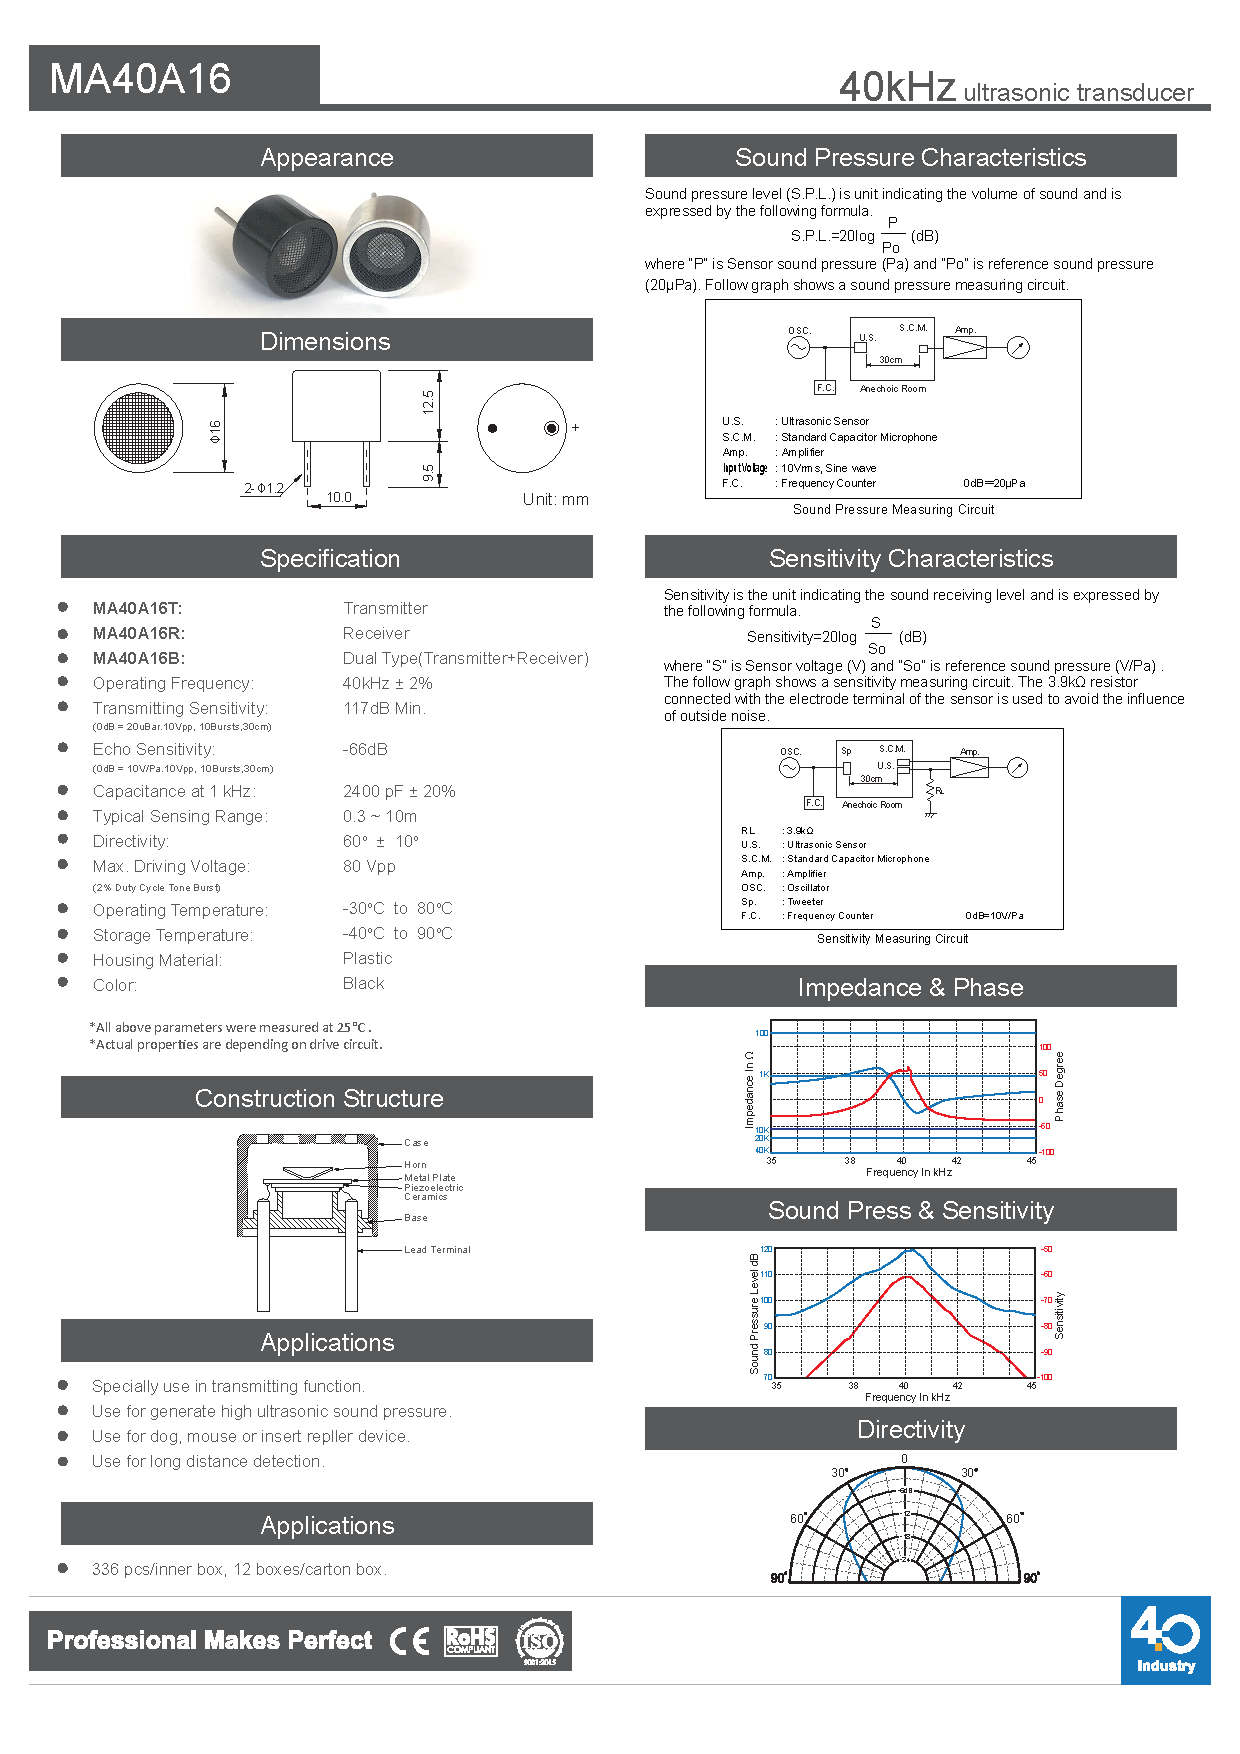
\includegraphics[angle=0, width=17.3cm, page=1]{appendix/MA40A16}}}
\end{adjustwidth}
\newpage

\section{Audio-Beamformer Schematics} \label{Fleet-Monitor V1.0 Schematics}
\enlargethispage{2.5cm}
\begin{adjustwidth}{0.23cm}{0cm} \hfuzz=7.0pt \vfuzz=20.0pt
\makebox[\textwidth]{\includegraphics[angle=90, width=17.3cm, page=1]{appendix/Audio-Beamformer.pdf}}
\end{adjustwidth}
\newpage

\begin{adjustwidth}{-0.23cm}{0cm} \hfuzz=7.0pt \vfuzz=20.0pt
\makebox[\textwidth]{\includegraphics[angle=90, width=17.3cm, page=2]{appendix/Audio-Beamformer.pdf}}
\end{adjustwidth}
\newpage

\begin{adjustwidth}{0.23cm}{0cm} \hfuzz=7.0pt \vfuzz=20.0pt
\makebox[\textwidth]{\includegraphics[angle=90, width=17.3cm, page=3]{appendix/Audio-Beamformer.pdf}}
\end{adjustwidth}
\newpage

\begin{adjustwidth}{-0.23cm}{0cm} \hfuzz=7.0pt \vfuzz=20.0pt
\makebox[\textwidth]{\includegraphics[angle=90, width=17.3cm, page=4]{appendix/Audio-Beamformer.pdf}}
\end{adjustwidth}
\newpage

\begin{adjustwidth}{0.23cm}{0cm} \hfuzz=7.0pt \vfuzz=20.0pt
\makebox[\textwidth]{\includegraphics[angle=90, width=17.3cm, page=5]{appendix/Audio-Beamformer.pdf}}
\end{adjustwidth}
\newpage

\begin{adjustwidth}{-0.23cm}{0cm} \hfuzz=7.0pt \vfuzz=20.0pt
\makebox[\textwidth]{\includegraphics[angle=90, width=17.3cm, page=6]{appendix/Audio-Beamformer.pdf}}
\end{adjustwidth}
\newpage

\begin{adjustwidth}{0.23cm}{0cm} \hfuzz=7.0pt \vfuzz=20.0pt
\makebox[\textwidth]{\includegraphics[angle=90, width=17.3cm, page=7]{appendix/Audio-Beamformer.pdf}}
\end{adjustwidth}
\newpage

\begin{adjustwidth}{-0.23cm}{0cm} \hfuzz=7.0pt \vfuzz=20.0pt
\makebox[\textwidth]{\includegraphics[angle=90, width=17.3cm, page=8]{appendix/Audio-Beamformer.pdf}}
\end{adjustwidth}
\newpage

\begin{adjustwidth}{0.23cm}{0cm} \hfuzz=7.0pt \vfuzz=20.0pt
\makebox[\textwidth]{\includegraphics[angle=90, width=17.3cm, page=9]{appendix/Audio-Beamformer.pdf}}
\end{adjustwidth}
\newpage

\begin{adjustwidth}{-0.23cm}{0cm} \hfuzz=7.0pt \vfuzz=20.0pt
\makebox[\textwidth]{\includegraphics[angle=90, width=17.3cm, page=10]{appendix/Audio-Beamformer.pdf}}
\end{adjustwidth}
\newpage

\section{PCB Top-Layer}
\enlargethispage{2.5cm}
\begin{adjustwidth}{0.23cm}{0cm} \hfuzz=7.0pt \vfuzz=19.0pt
\makebox[\textwidth]{\frame{\includegraphics[width=17.3cm, trim=75mm 12mm 67mm 6mm, clip, page=11]{appendix/Audio-Beamformer.pdf}}}
\end{adjustwidth}
\newpage

\section{PCB Bottom-Layer}
\enlargethispage{2.5cm}
\begin{adjustwidth}{-0.23cm}{0cm} \hfuzz=7.0pt \vfuzz=19.0pt
\makebox[\textwidth]{\frame{\includegraphics[width=17.3cm, trim=67mm 12mm 75mm 6mm, clip, page=12]{appendix/Audio-Beamformer.pdf}}}
\end{adjustwidth}
\newpage

\section{PCB Top-Overlay}
\enlargethispage{2.5cm}
\begin{adjustwidth}{0.23cm}{0cm} \hfuzz=7.0pt \vfuzz=19.0pt
\makebox[\textwidth]{\frame{\includegraphics[width=17.3cm, trim=75mm 12mm 67mm 6mm, clip, page=13]{appendix/Audio-Beamformer.pdf}}}
\end{adjustwidth}
\newpage

\section{PCB Bottom-Overlay}
\enlargethispage{2.5cm}
\begin{adjustwidth}{-0.23cm}{0cm} \hfuzz=7.0pt \vfuzz=19.0pt
\makebox[\textwidth]{\frame{\includegraphics[width=17.3cm, trim=67mm 9mm 75mm 6mm, clip, page=14]{appendix/Audio-Beamformer.pdf}}}
\end{adjustwidth}
\newpage

\section{PCB Outline}
\enlargethispage{2.5cm}
\begin{adjustwidth}{0.23cm}{0cm} \hfuzz=7.0pt \vfuzz=19.0pt
\makebox[\textwidth]{\frame{\includegraphics[width=17.3cm, trim=65.5mm 1mm 67mm 0mm, clip, page=15]{appendix/Audio-Beamformer.pdf}}}
\end{adjustwidth}
\newpage


\section{Bill of Materials (BOM)}
\enlargethispage{2.5cm}
\begin{adjustwidth}{-0.23cm}{0cm} \hfuzz=7.0pt \vfuzz=20.0pt
\makebox[\textwidth]{\includegraphics[width=17.3cm, trim=45mm 104mm 64mm 76mm, clip]{appendix/Audio-Beamformer BOM.pdf}}
\end{adjustwidth}
\newpage


\section{Mechanical Drawing Top-Plate}
\enlargethispage{2.5cm}
\begin{adjustwidth}{0.23cm}{0cm} \hfuzz=7.0pt \vfuzz=20.0pt
\makebox[\textwidth]{\includegraphics[angle=90, width=17.3cm]{appendix/Topplate.pdf}}
\end{adjustwidth}
\newpage

\section{Mechanical Drawing Base-Plate}
\enlargethispage{2.5cm}
\begin{adjustwidth}{-0.23cm}{0cm} \hfuzz=7.0pt \vfuzz=20.0pt
\makebox[\textwidth]{\includegraphics[angle=90, width=17.3cm]{appendix/Baseplate.pdf}}
\end{adjustwidth}
\newpage

\section{Mechanical Drawing Connecting-Bar}
\enlargethispage{2.5cm}
\begin{adjustwidth}{0.23cm}{0cm} \hfuzz=7.0pt \vfuzz=20.0pt
\makebox[\textwidth]{\includegraphics[angle=90, width=17.3cm]{appendix/Connecting-Bar.pdf}}
\end{adjustwidth}
\newpage






%\newpage


\iffalse


\section{Fleet-Monitor V1.0 BOM} \label{Fleet-Monitor V1.0 BOM}
\enlargethispage{1.6cm}
\begin{adjustwidth}{-0.23cm}{0cm} \hfuzz=7.0pt \vfuzz=20.0pt
\makebox[\textwidth]{\includegraphics[angle=90, width=16.5cm]{appendix/Fleet-Monitor_BOM_croped}}
\end{adjustwidth}
\newpage


\section{Fleet-Monitor V1.0 PCB Layout} \label{Fleet-Monitor V1.0 PCB Layout}
\enlargethispage{2.5cm}
\begin{adjustwidth}{0.23cm}{0cm} \hfuzz=7.0pt \vfuzz=20.0pt
\makebox[\textwidth]{\includegraphics[angle=90, width=17.3cm, page=1]{appendix/Fleet-Monitor Layout}}
\end{adjustwidth}
\newpage

\begin{adjustwidth}{-0.23cm}{0cm} \hfuzz=7.0pt \vfuzz=20.0pt
\makebox[\textwidth]{\includegraphics[angle=90, width=17.3cm, page=2]{appendix/Fleet-Monitor Layout}}
\end{adjustwidth}
\newpage

\begin{adjustwidth}{0.23cm}{0cm} \hfuzz=7.0pt \vfuzz=20.0pt
\makebox[\textwidth]{\includegraphics[angle=90, width=17.3cm, page=3]{appendix/Fleet-Monitor Layout}}
\end{adjustwidth}
\newpage

\begin{adjustwidth}{-0.23cm}{0cm} \hfuzz=7.0pt \vfuzz=20.0pt
\makebox[\textwidth]{\includegraphics[angle=90, width=17.3cm, page=4]{appendix/Fleet-Monitor Layout}}
\end{adjustwidth}
\newpage

\begin{adjustwidth}{0.23cm}{0cm} \hfuzz=7.0pt \vfuzz=20.0pt
\makebox[\textwidth]{\includegraphics[angle=90, width=17.3cm, page=5]{appendix/Fleet-Monitor Layout}}
\end{adjustwidth}
\newpage

\begin{adjustwidth}{-0.23cm}{0cm} \hfuzz=7.0pt \vfuzz=20.0pt
\makebox[\textwidth]{\includegraphics[angle=90, width=17.3cm, page=6]{appendix/Fleet-Monitor Layout}}
\end{adjustwidth}
\newpage


\section{Fleet-Monitor V1.0 Mechanical Drawing} \label{Fleet-Monitor V1.0 Mechanical Drawing}
\enlargethispage{2.5cm}
\begin{adjustwidth}{0.23cm}{0cm} \hfuzz=7.0pt \vfuzz=20.0pt
\makebox[\textwidth]{\includegraphics[angle=90, width=17.3cm, page=1]{appendix/Fleet-Monitor Case Drawing}}
\end{adjustwidth}
\newpage

\fi





\backmatter

\bibliographystyle{plain}
\typeout{}
\bibliography{./sections/bibliography.bib}

\end{document}